\documentclass{ieeeaccess}
\usepackage{cite}
\usepackage{amsmath,amssymb,amsfonts}
\usepackage{algorithmic}
\usepackage{graphicx}
\usepackage{textcomp}

\usepackage[ruled,noend,linesnumbered]{algorithm2e}
\usepackage{graphicx,color,psfrag}
\usepackage{amsmath}
\usepackage{amsfonts}
\usepackage{amssymb}
\usepackage{bigdelim}
\usepackage{dsfont}
\usepackage{color, soul}
\usepackage{caption}
\usepackage{subcaption}
\usepackage{url}
\usepackage{array,multirow,graphicx}
\usepackage{makecell}

\def\BibTeX{{\rm B\kern-.05em{\sc i\kern-.025em b}\kern-.08em
    T\kern-.1667em\lower.7ex\hbox{E}\kern-.125emX}}
\begin{document}
\history{Date of publication xxxx 00, 0000, date of current version xxxx 00, 0000.}
\doi{10.1109/ACCESS.20xx.0000000}

\title{Unsupervised Geometric-guided Industrial Anomaly Detection}

\author{\uppercase{Dinh-Cuong Hoang}\authorrefmark{1},
\uppercase{Phan Xuan Tan}\authorrefmark{2},
\uppercase{Anh-Nhat Nguyen}\authorrefmark{3},
\uppercase{Duc-Thanh Tran}\authorrefmark{3}
\uppercase{Van-Hiep Duong}\authorrefmark{3},
\uppercase{Anh-Truong Mai}\authorrefmark{3},
\uppercase{Duc-Long Pham}\authorrefmark{3},
\uppercase{Khanh-Toan Phan}\authorrefmark{3},
\uppercase{Minh-Quang Do}\authorrefmark{3},
\uppercase{Ta Huu Anh Duong}\authorrefmark{1},
\uppercase{Tuan-Minh Huynh}\authorrefmark{1},
\uppercase{Son-Anh Bui}\authorrefmark{1},
\uppercase{Duc-Manh Nguyen}\authorrefmark{1},
\uppercase{Viet-Anh Trinh}\authorrefmark{1}, and
\uppercase{Khanh-Duong Tran}\authorrefmark{1}}


\address[1]{Greenwich Vietnam, FPT University, Hanoi, 10000, Vietnam}
\address[2]{College of Engineering, Shibaura Institute of Technology, Tokyo 135-8548, Japan}
\address[3]{IT Department, FPT University, Hanoi, 10000, Vietnam}

%\tfootnote{This paragraph of the first footnote will contain support
%information, including sponsor and financial support acknowledgment. For
%example, ``This work was supported in part by the U.S. Department of
%Commerce under Grant BS123456.''}

\markboth
{D. C. Hoang \headeretal: Geometric-guided industrial anomaly detection}
{D. C. Hoang \headeretal: Geometric-guided industrial anomaly detection}

\corresp{Corresponding author: Xuan-Tan Phan (e-mail: tanpx@shibaura-it.ac.jp).}


\begin{abstract}

Industrial anomaly detection involves identifying abnormal regions in products and plays a crucial role in quality inspection. While 2D image-based anomaly detection has been extensively explored, combining two-dimensional (2D) images with three-dimensional (3D) point clouds remains less studied. Existing multimodal methods often combine features from different modalities, leading to feature interference and degraded performance. To overcome this, we propose a novel framework for unsupervised industrial anomaly detection that leverages both visual and geometric information. Specifically, we use pre-trained 2D and 3D models to extract visual features from color images and geometric features from 3D point clouds. Instead of directly fusing these features, we propose a geometric feature reconstruction network that predicts 3D geometric features from the 2D visual features. During training, we minimize the difference between the predicted geometric features and the extracted geometric features, enabling the model to learn how 2D appearance correlates with 3D structure in anomaly-free images. During inference, this learned relationship allows the model to detect anomalies: significant discrepancies between the reconstructed and actual geometric features indicate abnormal regions. Evaluated on the MVTec 3D-AD dataset, our method achieves state-of-the-art performance with an average image-level AUROC score of 0.968, surpassing previous approaches. Additionally, it provides fast inference at 8.2 frames per second with a memory footprint of only 1045 MB, making it highly efficient for industrial applications. 

\end{abstract}

\begin{keywords}
Industrial anomaly detection, image-based anomaly detection, 3D point clouds.
\end{keywords}

\titlepgskip=-21pt

\maketitle

%%%%%%%%%%%%%%%%%%%%%%%%%%%%%%%%%%%%%%%%%%%%%%%%%%%%%%%%%%%%%%%%%%%%

\section*{Introduction}

Industrial anomaly detection (IAD) plays an important role for ensuring quality control and minimizing defects in manufacturing processes \cite{chandola2009anomaly, iturbe2017towards, prunella2023deep}. It can be integrated into automation systems \cite{hoang2024graspability, cui2023survey, vu2024occlusion} to monitor production lines, detect irregularities in real-time, and enable adaptive decision-making \cite{bergmann2020uninformed, hoang2019object, liu2020towards, hoang2022context}. Early detection of anomalies, often caused by equipment malfunctions or material defects, is crucial for mitigating financial losses and operational disruptions \cite{ren2024steel, zhang2024defect}. Traditional methods for detecting these anomalies relied heavily on filtering and handcrafted features to distinguish between normal and abnormal samples \cite{chandola2009anomaly}. However, these approaches often perform poorly with complex and high-dimensional data, such as industrial images \cite{yang2019real}.

With the advent of deep learning, anomaly detection techniques have evolved significantly \cite{tao2022deep, cui2023survey}. In particular, unsupervised methods have gained attention due to the challenges and costs associated with obtaining labeled data for abnormal instances \cite{cui2023survey}. These methods typically train models using only normal samples, enabling the system to identify deviations from normality in unseen test samples that may contain both normal and abnormal data. Deep learning-based anomaly detection techniques primarily focus on two categories: reconstruction-based and feature-embedding methods. Reconstruction-based methods aim to restore anomalous regions by comparing reconstructed images with the originals, thus highlighting discrepancies at defect locations \cite{akcay2019ganomaly, yu2023unsupervised, liu2020towards}. Despite their success in detecting anomalies, these methods often struggle with the extraction of high-level semantic features, which limits their classification performance. On the other hand, feature-embedding methods leverage pre-trained networks to learn representations of normal samples \cite{bergmann2020uninformed, salehi2021multiresolution, wang2021student, cao2022informative}. Deviations from these learned representations signal the presence of anomalies. These methods often adopt a teacher-student architecture, where a backbone model serves as a teacher to train a student model for feature extraction. Anomaly detection is then performed by comparing feature maps from both models, with significant deviations indicating anomalies.

While the above techniques have proven effective, they often rely on RGB image data, which lacks the geometric context necessary for precise anomaly localization in industrial settings. Recent advancements in computer vision have explored the use of depth images and 3D point clouds to enhance detection by capturing geometric cues alongside traditional RGB features \cite{bergmann2023anomaly, rudolph2023asymmetric, horwitz2023back, wang2023multimodal}. However, despite the potential of these multimodal approaches, several limitations remain. First, the high-dimensionality of 3D point cloud data, coupled with the irregularity of point clouds, presents a significant challenge for traditional convolutional neural networks (CNNs), which are primarily designed for structured data \cite{hoang2025attention, wang2023multimodal, hoang2024efficient}. Another limitation lies in the computational complexity and resource demands of multimodal methods \cite{rudolph2023asymmetric, hoang2024collision}. Processing high-resolution depth maps or point clouds alongside RGB images requires substantial memory and processing power, which can make real-time industrial applications impractical \cite{horwitz2023back, hoang2024object}. Memory-based methods, for example, store representative features from both modalities, but their reliance on large feature banks increases memory requirements and prolongs inference times, hindering their deployment in resource-constrained environments.

In this paper,  we propose an unsupervised anomaly detection framework that effectively leverages both visual and geometric information. Our approach begins by using pre-trained transformer-based models to separately extract 2D visual features from color images and 3D geometric features from point clouds. We then design a Visual-to-Geometric Feature Reconstruction network that takes the visual features as input and predicts the corresponding geometric features. Through the use of non-local attention mechanisms, the model captures global relationships between visual and geometric features, ensuring that long-range dependencies in the data are retained, while graph convolutional networks (GCNs) enable it to refine local geometric details by modeling high-order spatial relationships between neighboring visual tokens. During training, the network minimizes the difference between the predicted geometric features and the original geometric features extracted from the point cloud, which enables it to learn the correlation between appearance and geometry in normal objects. By focusing on reconstructing the geometric features based on visual inputs, the network captures how normal visual features translate into geometric representations, making it highly responsive to any anomalies in the test data. Since the training data contains only normal samples, the network learns the expected patterns and correlations between 2D and 3D features for normal objects. During inference, any significant deviation between the predicted and actual geometric features signals the presence of an anomaly.

In brief, the main contributions of our work are:

\begin{itemize}
    \item \textbf{Innovative Anomaly Detection Network}: We propose a novel unsupervised anomaly detection framework that reconstructs 3D geometric features from 2D visual features using a geometric feature prediction network, rather than directly fusing the modalities.
     
    \item \textbf{Visual-to-Geometric Feature Reconstruction}: The core innovation of our framework lies in the introduction of a visual-to-geometric feature reconstruction network, which predicts 3D geometric features from 2D visual inputs. This approach leverages two key techniques: (1) non-local attention mechanisms and (2) graph convolution networks (GCNs) to effectively capture both global and local relationships between 2D and 3D features.
     
    \item \textbf{Training Strategy}: We introduce a training strategy to minimize the difference between the predicted geometric features and the target geometric features extracted from point clouds, allowing the network to learn the normal correlations between 2D and 3D features.
    
    \item \textbf{State-of-the-Art Performance}: Our method demonstrates state-of-the-art performance on industrial anomaly detection tasks, with significant improvements in both detection accuracy and inference speed.
\end{itemize}
 
%
\section*{Related work}
\label{sec:relatedwork}

\subsection*{Unsupervised anomaly detection}

The majority of recent research on industrial anomaly detection has focused on unsupervised methods due to the challenges and costs associated with collecting labeled abnormal samples. Typically, only normal samples are used in the training set, while both normal and abnormal samples are included in the test set. Before the advent of deep learning, traditional techniques such as differential detection and filtering were frequently used to identify anomalies in industrial images. With the rise of deep learning, anomaly detection methods for industrial images have largely shifted toward two main categories: reconstruction-based and feature-embedding methods.

\subsubsection*{Reconstruction-Based Methods}

The core assumption of reconstruction-based methods is that the model should be able to restore anomalous regions by comparing the reconstructed image to the original. Differences at the anomalous positions enable defect localization. During training, normal or abnormal images are fed into the reconstruction network, with the reconstruction loss function guiding the network’s learning process. The trained network is then expected to restore images resembling the original normal images. During inference, a comparison model highlights the discrepancies between the original and reconstructed images to make predictions. Early models include Auto-Encoder (AE) \cite{yu2023unsupervised, collin2021improved}, Variational Auto-Encoder (VAE) \cite{liu2020towards}, and Generative Adversarial Networks (GAN) \cite{akcay2019ganomaly, perera2019ocgan}. For example, \cite{bergmann2018improving} explores how the structure similarity index measure (SSIM) affects AE reconstruction and anomaly segmentation. To avoid over-detection, \cite{chung2020unsupervised} propose the Outlier-Exposed Style Distillation Network (OE-SDN), which focuses on maintaining style translation while limiting content translation in the AE. Structural improvements to AE have also been explored. For instance, \cite{zhou2020encoding} introduced P-Net to compare structural differences between the original and reconstructed images, while \cite{collin2021improved} incorporated skip-connections between the encoder and decoder to enhance reconstruction sharpness.

VAEs are a variation of AEs, differing in that VAE's intermediate variables are sampled from a normal distribution \cite{liu2020towards, dehaene2020iterative}. To address VAE's tendency to produce blurry reconstructions, \cite{dehaene2020iterative} introduced gradient descent in reconstruction with energy defined by the reconstruction loss, preserving high-frequency structures. FAVAE \cite{dehaene2020anomaly} models the distribution of features extracted by pre-trained models, enabling the detection of a broader range of anomalies and enhancing generalization. VQ-VAE \cite{wang2020image} adds a discrete latent space and resamples the latent codes deviating from normal distributions, improving reconstruction by focusing on closer-to-normal images. 

Reconstruction models based on GANs have been shown to be less stable than AE-based models, but the discriminative power of GAN’s networks can be more effective in specific contexts. SCADN (Semantic Context-based Anomaly Detection Network) \cite{yan2021learning} masks parts of the image during training and reconstructs them using GAN, detecting anomalies by comparing the reconstructed and original images. AnoSeg \cite{song2021anoseg} uses hard augmentation, adversarial learning, and channel concatenation to generate abnormal samples and trains GAN to generate normal samples, incorporating both reconstruction loss and adversarial loss in its objective function. OCR-GAN \cite{liang2023omni} decouples an image into various frequency components and reconstructs them separately, improving anomaly detection. However, while reconstruction-based methods are effective in anomaly detection, their classification performance is limited due to a weaker ability to extract high-level semantic features.

\subsubsection*{Feature-Embedding Methods}

In contrast, feature-embedding methods rely on pre-trained feature extractors to identify anomalies \cite{rudolph2021same, wang2021student}. Features from normal samples typically conform to a known distribution, and deviations from this distribution signal anomalies. Several studies \cite{bergmann2020uninformed, salehi2021multiresolution, wang2021student, cao2022informative} adopt a teacher-student architecture for anomaly detection. In this approach, a backbone network pre-trained on a large-scale dataset serves as the teacher model, which is then used to train the student model to extract features from normal samples. During inference, normal image features from the test set extracted by both networks are similar, but features from abnormal images differ significantly. An anomaly score map is generated by comparing the feature maps from both networks, and when scaled to the input image size, this map indicates the anomaly scores of various regions. Some researchers have framed anomaly detection as a one-class classification (OCC) problem, inspiring enhancements to traditional methods like Support Vector Data Description (SVDD) \cite{tax2004support, defard2021padim}. For example, \cite{yi2021patch, zhang2021anomaly, hu2021semantic} have adapted SVDD for industrial anomaly detection. Another approach leverages memory banks \cite{cohen2020sub, li2021anomaly, wan2021industrial, roth2022towards} to store representative features. These memory-based methods require minimal network training, relying on pre-sampled normal features for inference. During inference, features from the test image are compared with those in the memory bank, and the distance from the normal features determines the anomaly probability \cite{lee2022cfa, kim2023fapm, defard2021padim}. However, while memory-based methods can be efficient, they tend to have higher memory requirements and longer inference times due to the storage of representative.

\subsection*{Anomaly Detection with Dual Modalities}

RGB images provide rich semantic information, while depth images or point clouds capture essential geometric cues. Many studies have explored how to leverage the complementary nature of these data types across various computer vision tasks. Recently, depth data (or 3D information) has been utilized to improve the robustness and accuracy of anomaly detection systems \cite{horwitz2022empirical, wang2023multimodal}. \cite{bergmann2023anomaly} introduced the 3D Student-Teacher (3D-ST) model for unsupervised anomaly detection, which operates directly on 3D point clouds. This method, trained solely on anomaly-free data, identifies geometric anomalies in high-resolution test samples with just a single forward pass. However, the method's effectiveness is limited by the similarity between the student and teacher networks, which leads to small distances even for anomalies. To address this, \cite{rudolph2023asymmetric} proposed Asymmetric Student-Teacher networks (AST), where a normalizing flow model is used as the teacher for density estimation, while a conventional feed-forward network serves as the student. This architecture induces larger distances for anomalies. The AST approach is extendable to multimodal inputs, including RGB and 3D data, by concatenating depth maps with RGB features along the channels when 3D data is available. Horwitz et al. \cite{horwitz2023back} explored the integration of geometric features with visual features for anomaly detection, examining a wide range of both hand-crafted and deep learning-based representations. Their findings indicated that hand-crafted descriptors from point clouds provided the most effective results. Building on this, Wang et al. \cite{wang2023multimodal} enhanced the approach by utilizing more informative visual and geometric features extracted from pre-trained models on large datasets. They introduced a learned function to fuse visual and geometric features into unified multimodal representations, which were stored in memory banks along with features from each individual modality. However, this method's dependence on extensive feature banks made it resource-intensive. In contrast to these approaches, our proposed method does not fuse visual and geometric features directly. Instead, it learns to map visual features to their corresponding geometric features. By reconstructing geometric features from visual inputs using pre-trained models, our approach significantly reduces memory usage and enhances inference speed, while maintaining high effectiveness in anomaly detection.
%
\section*{Methodology}

\begin{figure*}[ht]
\centering
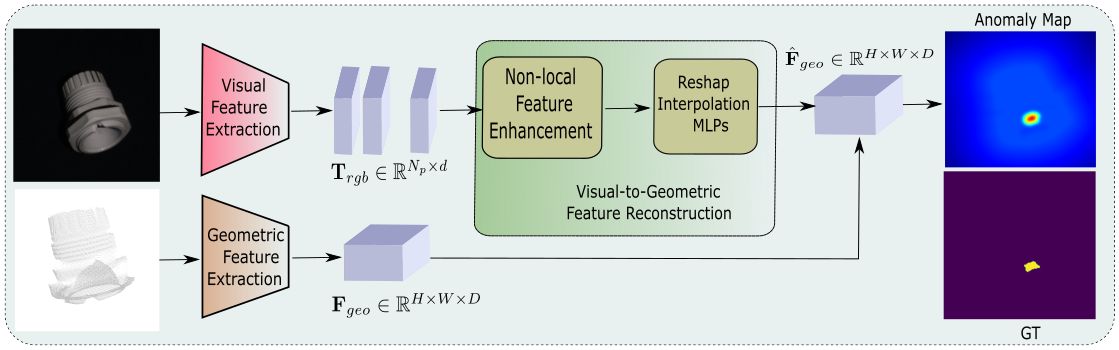
\includegraphics[width=\linewidth]{figs/overview}
\caption{Overview of the proposed unsupervised anomaly detection framework. The method extracts 2D visual features from RGB images and 3D geometric features from point clouds. A Visual-to-Geometric Feature Reconstruction network predicts geometric features from visual inputs, and significant discrepancies indicate anomalies.}
\label{fig:view}
\end{figure*}

Let $\mathbf{I} \in \mathbb{R}^{H \times W \times 3}$ represent an RGB image, where $H$ and $W$ denote the height and width of the image, and the 3 channels correspond to the color information. Let $\mathbf{D} \in \mathbb{R}^{H \times W}$ represent the corresponding depth image, which is pixel-registered with $\mathbf{I}$. This means that each pixel $(u, v)$ in $\mathbf{D}$ corresponds to a pixel in $\mathbf{I}$, providing a depth value $d_{u,v}$ for each valid pixel. From the depth image $\mathbf{D}$, we generate a 3D point cloud $\mathbf{P} = \{(x_i, y_i, z_i)\}_{i=1}^{M}$, where $M$ is the number of valid depth points and each point $(x_i, y_i, z_i)$ represents the 3D coordinates derived from the depth information.

As shown in Figure \ref{fig:view} the objective of the proposed method is to detect anomalies by predicting the 3D geometric features $\hat{\mathbf{F}}_{geo}$ from the 2D visual features $\mathbf{F}_{vis}$ and comparing them with the actual geometric features $\mathbf{F}_{geo}$ extracted from the point cloud. First, the visual features $\mathbf{F}_{vis} \in \mathbb{R}^{H \times W \times d}$ are extracted from the RGB image $\mathbf{I}$ using a Vision Transformer (ViT), capturing the appearance of the object in 2D space. Then, the 3D geometric features $\mathbf{F}_{geo} \in \mathbb{R}^{H \times W \times d}$ are obtained from the depth image $\mathbf{D}$ using a pre-trained 3D model. The core of the method is the geometric feature reconstruction network, which predicts the geometric features $\hat{\mathbf{F}}_{geo}$ from the visual inputs $\mathbf{F}_{vis}$. During training, the network minimizes the difference between the predicted geometric features $\hat{\mathbf{F}}_{geo}$ and the actual geometric features $\mathbf{F}_{geo}$ by minimizing the loss $\mathcal{L}_{geo}$. This process allows the network to learn the normal correlations between 2D visual data and 3D geometric data. During inference, anomalies are detected by comparing the predicted geometric features $\hat{\mathbf{F}}_{geo}$ with the actual geometric features $\mathbf{F}_{geo}$. Significant deviations between these features, measured using the Euclidean distance or another discrepancy measure, indicate abnormal regions in the object.

\subsection*{3D Point Cloud Feature Extraction}

The 3D point cloud $\mathbf{P} = \{(x_i, y_i, z_i)\}_{i=1}^{M}$ is processed using a Masked Autoencoder (MAE) \cite{pang2022masked}. The point cloud is first divided into patches using Farthest Point Sampling (FPS) and K-Nearest Neighbors (KNN). FPS selects $n$ points as patch centers, and KNN selects the $k$ nearest neighbors for each center:

\begin{equation}
    \mathbf{C_T} = \text{FPS}(\mathbf{P}), \quad \mathbf{C_T} \in \mathbb{R}^{n \times 3}
\end{equation}
\begin{equation}
    \mathbf{P}_{patch} = \text{KNN}(\mathbf{P}, \mathbf{C_T}), \quad \mathbf{P}_{patch} \in \mathbb{R}^{n \times k \times 3}
\end{equation}

\noindent The masked point patches are processed through PointNet \cite{qi2017pointnet} and the autoencoder to produce geometric features $\mathbf{G}_{geom} \in \mathbb{R}^{M \times D}$. The geometric features $\mathbf{G}_{geom} \in \mathbb{R}^{M \times d}$ are produced for each point in the point cloud. Since the 3D point cloud is derived from the depth image $\mathbf{D}$, we know the pixel coordinates $(u_i, v_i)$ of each 3D point $(x_i, y_i, z_i)$, allowing us to map the geometric features back to their corresponding pixel locations in the 2D image. Using this projection, we place the geometric features into a sparse 2D feature map $\mathbf{G}_{map} \in \mathbb{R}^{H \times W \times d}$, where the pixel $(u_i, v_i)$ contains the feature vector for point $i$.

\begin{equation}
\mathbf{G}_{map}[u_i, v_i, :] = \mathbf{G}_{geom}[i, :]
\end{equation}

\noindent For pixels without corresponding 3D points, we apply interpolation method as in \cite{wang2023multimodal} to propagate geometric features from neighboring pixels:

\begin{equation}
    \mathbf{F}_{geo} = \text{Interpolate}(\mathbf{G}_{map}) \in \mathbb{R}^{H \times W \times D}
\end{equation}

\subsection*{Visual Feature Extraction}

The RGB image $\mathbf{I}$ is processed using a Vision Transformer (ViT) \cite{dosovitskiy2020image} to extract high-level visual features. The image $\mathbf{I}$ is divided into non-overlapping patches of size $p \times p$, and each patch is flattened into a vector. A linear projection is applied to embed the patches into a $d$-dimensional feature space:

\begin{equation}
    \mathbf{x}_p = \text{Flatten}(\mathbf{I}) \in \mathbb{R}^{(H \times W) / p^2 \times (p \times p \times 3)}
\end{equation}

\noindent The set of embedded patches is passed through the transformer encoder to obtain RGB feature tokens:

\begin{equation}
    \mathbf{T}_{rgb} = ViT(\mathbf{x}_p) \in \mathbb{R}^{N_p \times d}
\end{equation}

\noindent where $N_p = \frac{H \times W}{p^2}$ is the number of patches and $d$ is the dimension of the feature vectors. 

\subsection*{Visual-to-Geometric Feature Reconstruction}

\begin{figure*}[ht]
\centering
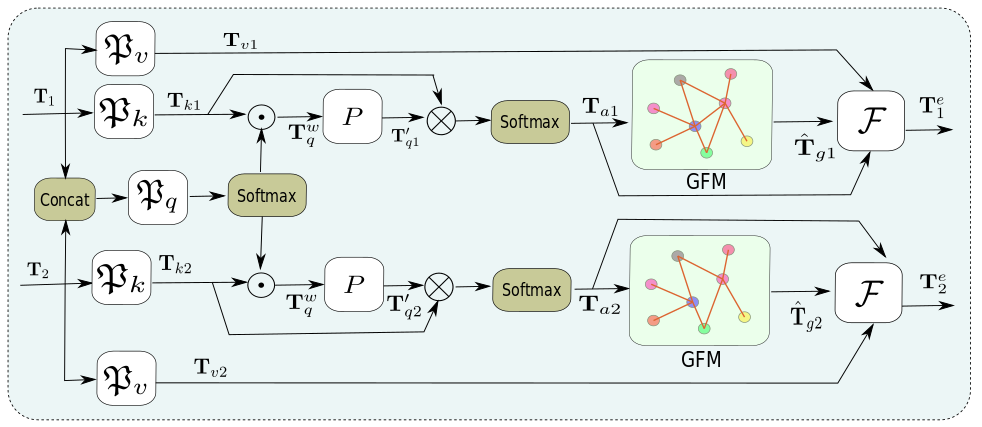
\includegraphics[width=0.8\linewidth]{figs/NL}
\caption{The proposed visual feature enhancement module $\mathcal{M}_{FE}$ used in geometric feature reconstruction. The module incorporates non-local attention and graph convolutional networks to improve the interaction between global and local features.}
\label{fig:NL}
\end{figure*}

The Visual-to-Geometric Feature Reconstruction network serves as the core of the proposed method, learning to reconstruct 3D geometric features from 2D visual inputs. This approach leverages the complementary nature of appearance and geometric information, enabling precise anomaly detection without the need for direct multimodal fusion. 

Transformers are well-suited for capturing global contextual information across visual tokens; however, their ability to model localized interactions remains limited. This limitation is particularly critical in anomaly detection, where fine-grained deviations often indicate defects. To address this, we integrate a visual feature enhancement module $\mathcal{M}_{FE}$ (Figure~\ref{fig:NL}) within the reconstruction network. This module enhances local feature representations while retaining global context by combining non-local attention \cite{wang2018non} with graph convolutional networks (GCNs) \cite{defferrard2016convolutional, te2020edge}. The combination of non-local attention and graph convolutional networks (GCNs) was chosen to effectively address the complementary aspects of global and local feature integration. Non-local attention captures long-range dependencies across the entire image, which is critical for identifying correlations in visual features across spatially distant regions. GCNs, on the other hand, excel at modeling local relationships and refining features based on neighborhood structures.

\paragraph*{Non-Local Attention for Global Context}
Non-local attention \cite{wang2018non} captures relationships between spatially distant visual tokens, providing the network with a global understanding of correlations in visual features. Specifically, given two neighboring tokens $\mathbf{T}_1$ and $\mathbf{T}_2$ extracted from a Vision Transformer, the attention mechanism refines $\mathbf{T}_1$ as follows:
\[
\mathbf{T}_v = \mathfrak{P}_v(\mathbf{T}_1), \quad \mathbf{T}_k = \mathfrak{P}_k(\mathbf{T}_1),
\]
where $\mathfrak{P}_v$ and $\mathfrak{P}_k$ are linear projection layers reducing the dimensionality of $\mathbf{T}_1$ to $\frac{d}{2}$. $\mathbf{T}_1$ and $\mathbf{T}_2$ are concatenated to form $\mathbf{T}_q$, and the attention weights are computed as:
\[
\mathbf{T}_q^w = \text{softmax}(\mathfrak{P}_q(\mathbf{T}_q)), \quad \mathbf{T}_q' = P\left(\mathbf{T}_k \odot \mathbf{T}_q^w\right),
\]
where $\mathfrak{P}_q$ projects $\mathbf{T}_q$ to a lower dimension, and $P(\cdot)$ is adaptive average pooling. The attention map $\mathbf{T}_a$ is derived from the interaction:
\[
\mathbf{T}_a = \text{softmax}(\mathbf{T}_q' \otimes \mathbf{T}_k^\top).
\]

\paragraph*{Graph Convolutional Networks for Local Interactions}
Local interactions between visual features are refined using a graph convolutional network (GCN) \cite{te2020edge}. Tokens are projected into a graph representation where vertices represent similar features, and edges encode relationships. The refined token $\hat{\mathbf{T}}_g$ is computed as:
\[
\hat{\mathbf{T}}_g = \text{ReLU}\left((I - A)\mathbf{T}_g w_g\right),
\]
where $\mathbf{T}_g = \mathbf{T}_v \otimes \mathbf{T}_a^\top$, $A$ is the adjacency matrix, and $w_g$ is the GCN weight matrix. A skip connection integrates global and local refinements:
\[
\mathbf{T}_1^e = \hat{\mathbf{T}}_g + \mathbf{T}_1.
\]

\noindent The same process is applied to other tokens. The adjacency matrix $A$ is dynamically constructed based on the similarity of visual tokens in the feature space. Specifically, token similarity is measured using a distance metric, and a thresholding mechanism is applied to determine graph connectivity. This approach ensures that $A$ adapts to the characteristics of each input, capturing relevant local relationships. The GCN's ability to model higher-order interactions and propagate contextual information across connected nodes provides a distinct advantage over simpler feature aggregation methods, particularly in capturing subtle anomalies that span localized regions.

\paragraph*{Reconstruction of Geometric Features}
The enhanced visual features $\mathbf{T}^e$ are reshaped and upsampled to match the spatial dimensions of the input image:
\[
\mathbf{F}_{patches} = \text{Reshape}(\mathbf{T}^e) \in \mathbb{R}^{\frac{H}{p} \times \frac{W}{p} \times d},
\]
\[
\mathbf{F}_{vis} = \text{BilinearUpsample}(\mathbf{F}_{patches}) \in \mathbb{R}^{H \times W \times d}.
\]
Bilinear upsampling was selected for its simplicity and computational efficiency. While more complex methods, such as learnable upsampling, could potentially improve alignment precision, experiments showed that bilinear upsampling produced negligible artifacts and did not significantly affect the accuracy of the reconstructed geometric features. Finally, $\mathbf{F}_{vis}$ is passed through a lightweight MLP to predict geometric features $\hat{\mathbf{F}}_{geo}$:
\[
\hat{\mathbf{F}}_{geo} = \text{MLP}(\mathbf{F}_{vis}).
\]

\paragraph*{Loss Function}
The network minimizes the L2 reconstruction loss to align the predicted geometric features $\hat{\mathbf{F}}_{geo}$ with the ground-truth features $\mathbf{F}_{geo}$:
\[
\mathcal{L}_{geo} = \frac{1}{HWD} \sum_{i=1}^{H} \sum_{j=1}^{W} \sum_{k=1}^{D} \left( \mathbf{F}_{geo}(i, j, k) - \hat{\mathbf{F}}_{geo}(i, j, k) \right)^2.
\]

By leveraging non-local attention and GCNs, $\mathcal{M}_{FE}$ ensures effective integration of global and local information. This design allows the network to capture subtle deviations in both texture and geometry, resulting in accurate anomaly detection for complex industrial settings.


\subsection*{Anomaly Localization}

During inference, we use the trained prediction network to predict geometric features from the visual features of test samples. For each sample, we extract the 2D visual features $\mathbf{F}_{vis}$ from the RGB image using the pre-trained 2D model and the 3D geometric features $\mathbf{F}_{geo}$ from the point cloud using the pre-trained 3D model. The visual features $\mathbf{F}_{vis}$ are then passed through the geometric feature prediction network to predict the corresponding geometric features $\hat{\mathbf{F}}_{geo}$. We compute an anomaly map by measuring the difference between the predicted geometric features $\hat{\mathbf{F}}_{geo}$ and the actual geometric features $\mathbf{F}_{geo}$ at each spatial location using the L2 norm:

\begin{equation}
\mathbf{A}_{\text{anomaly}}(i, j) = \|\mathbf{F}_{geo}(i, j) - \hat{\mathbf{F}}_{geo}(i, j)\|_2
\end{equation}

\noindent This anomaly map $\mathbf{A}_{\text{anomaly}} \in \mathbb{R}^{H \times W}$ indicates the likelihood of anomalies at each spatial location. Regions with higher values represent areas where the predicted geometric features deviate significantly from the actual geometric features, suggesting the presence of anomalies. The predicted anomaly map is finally smoothed using a Gaussian kernel with $\sigma$=4, following \cite{roth2022towards}. To obtain a global anomaly score for each sample, we calculate the maximum value in the smoothed anomaly map:

\begin{equation}
S_{\text{global}} = \max_{i,j} \mathbf{A}_{\text{anomaly}}(i, j)
\end{equation}

\noindent If the global anomaly score $S_{global}$ exceeds a predefined threshold, the sample is classified as anomalous. Additionally, the anomaly map provides spatial localization of anomalies by highlighting regions where the largest deviations occur, enabling a detailed inspection of the anomalous areas. 

%
\section*{Evaluation}
\label{sec:evaluation}

\begin{figure*}[ht]
\centering
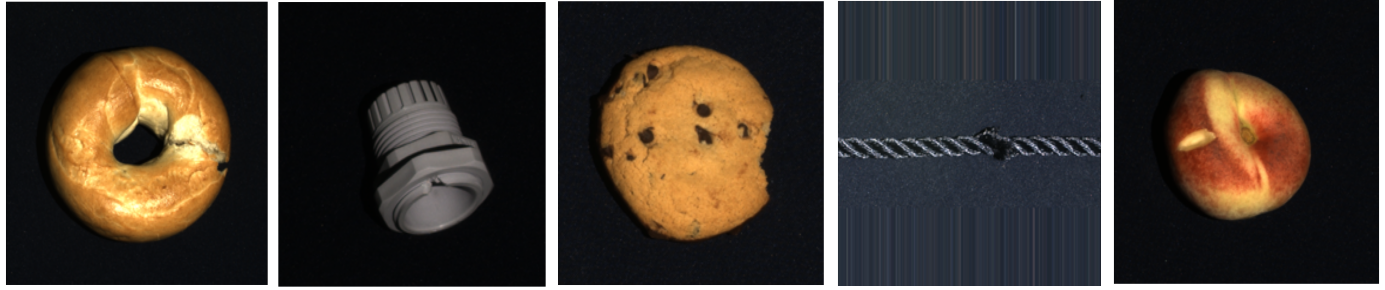
\includegraphics[width=\linewidth]{figs/result_rgb}
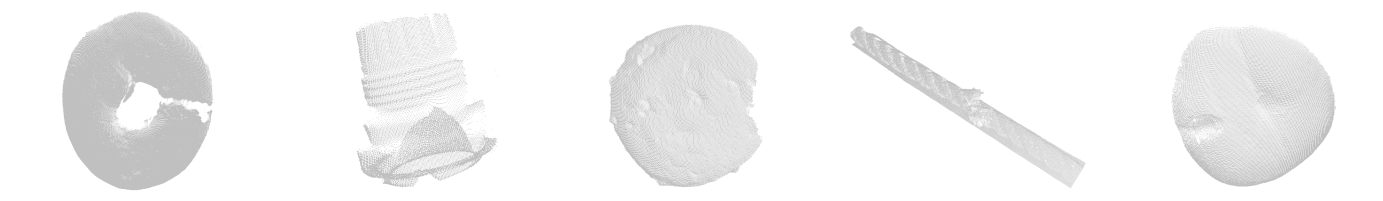
\includegraphics[width=\linewidth]{figs/result_pc}
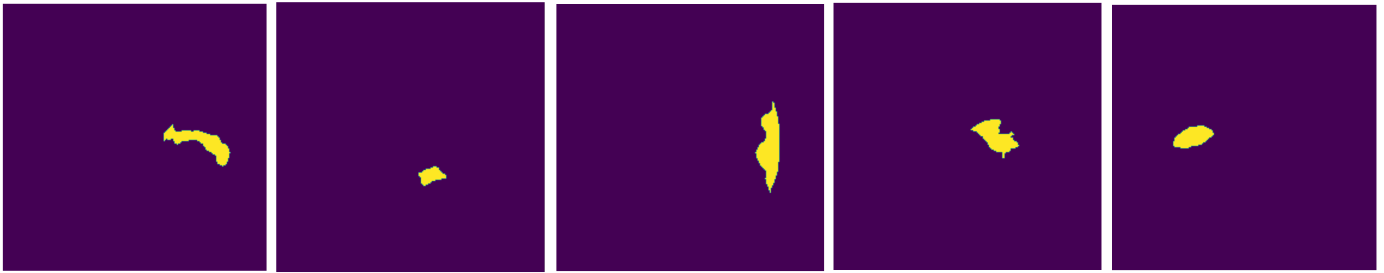
\includegraphics[width=\linewidth]{figs/result_gt}
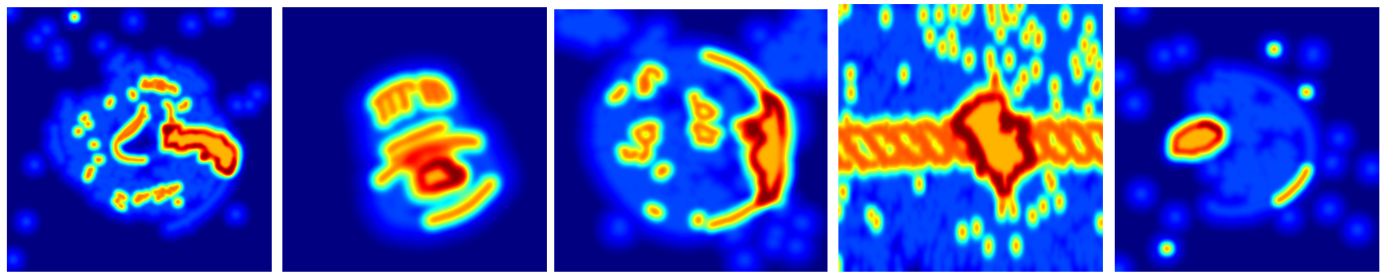
\includegraphics[width=\linewidth]{figs/result_baseline}
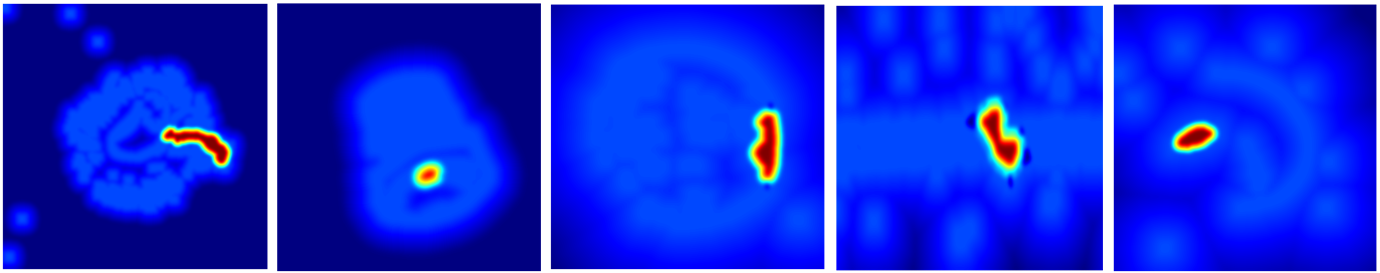
\includegraphics[width=\linewidth]{figs/result_ours}
\caption{Qualitative results of anomaly detection. From top to bottom: input RGB images, point clouds, ground-truth anomaly segmentations, anomaly maps from \cite{wang2023multimodal}, and anomaly maps obtained with our proposed method.}
\label{fig:results}
\end{figure*}

\subsection*{Experimental Details}

\textbf{Dataset.}  Most existing industrial anomaly detection datasets provides 2D RGB images without corresponding 3D point cloud data. In contrast, 3D industrial anomaly detection is still in its early stages. The MVTec 3D-AD dataset \cite{bergmann2022mvtec} is the first 3D dataset for industrial anomaly detection. Following previous works \cite{wang2023multimodal}, we conduct our experiments on this dataset, which is designed to reflect real-world industrial inspection scenarios. The dataset includes 10 categories of industrial objects, comprising 2656 training samples, 294 validation samples, and 1197 test samples. The 3D scans were captured using a structured light-based industrial sensor, where the position information is stored in three-channel tensors representing x, y, and z coordinates. Each sample includes both RGB images and pixel-registered 3D information, providing a rich dataset for experiments. The object categories vary from items with natural variations (e.g., bagels, carrots, peaches) to more rigid and structured items (e.g., cable glands, dowels). The test set contains simulated real-world defects such as scratches, dents, holes, contaminations, and deformations, with ground-truth annotations provided for each anomalous sample. \\

\noindent \textbf{Implementation Details.} Following \cite{wang2023multimodal}, we apply the RANSAC algorithm \cite{fischler1981random} to estimate the background plane, discarding any points within a distance of 0.005 units. For feature extraction, we utilize frozen Transformers as in \cite{wang2023multimodal}. Specifically, we employ DINO ViT-B/8 \cite{dosovitskiy2020image} pre-trained on ImageNet \cite{deng2009imagenet} for visual feature extraction, and Point-MAE \cite{pang2022masked} pre-trained on ShapeNet \cite{chang2015shapenet} for geometric feature extraction. The visual feature extraction module processes RGB images of resolution $224 \times 224$, producing a $28 \times 28 \times 768$ feature map, which is then upsampled to $224 \times 224 \times 768$ using bilinear interpolation before being passed to the geometric feature reconstruction module. For the point cloud data, we sample 1024 groups of 32 points using Farthest Point Sampling (FPS) \cite{qi2017pointnet++}, yielding a $1152$-dimensional feature vector for each group. These feature vectors are interpolated and aligned to a $224 \times 224 \times 1152$ grid, which serves as the target geometric feature map for reconstruction. The geometric feature reconstruction module is composed of three fully connected layers with GeLU activation functions applied after the first two layers. The layers have 768, 960, and 1152 units, respectively. We train the network for 200 epochs using the Adam optimizer \cite{kingma2014adam} with a learning rate of 0.001. All experiments are conducted on a single NVIDIA GeForce RTX 4090 GPU, utilizing both our implementation and the original authors' code for comparison. \\

\noindent \textbf{Evaluation Metrics.} Following \cite{bergmann2022mvtec, wang2023multimodal}, we employ two metrics: the Image-level Area Under the Receiver Operating Characteristic curve (I-AUROC) and the Area Under the Per-Region Overlap curve (AUPRO). These metrics provide insights into both anomaly classification and localization performance. I-AUROC is used to assess the model's ability to classify an entire test image as either anomaly-free or containing an anomaly. The AUROC curve is derived by plotting the true positive rate (TPR) against the false positive rate (FPR) at various threshold levels. The I-AUROC score provides a threshold-independent evaluation of the model's classification performance, with a score of 1 indicating perfect classification. A higher I-AUROC score signifies better image-level anomaly detection performance. AUPRO evaluates the model's ability to localize anomalies within the test samples. AUPRO measures how well the predicted anomaly regions overlap with the ground truth at different thresholds, thus reflecting the model's localization accuracy. For each connected component \( C_k \) in the ground truth, the overlap between the binary prediction \( P \) and \( C_k \) is computed. The Per-Region Overlap (PRO) for each region is defined as:
\begin{equation}
    \text{PRO}(C_k) = \frac{|P \cap C_k|}{|C_k|}
\end{equation}
AUPRO is computed by integrating the PRO over a range of thresholds, typically up to a false positive rate (FPR) limit.  We report the area under the PRO curve with an upper integration limit of 0.3 as in \cite{bergmann2022mvtec}. By focusing on localization performance, AUPRO offers a more precise evaluation of anomaly detection in complex industrial settings, where accurately pinpointing defect regions is critical. These metrics together provide a comprehensive view of the model's ability to detect and localize anomalies.

\subsection*{Results}

\begin{table*}[ht]
\centering
\begin{tabular}{cl|r|r|r|r|r|r|r|r|r|r|r}
\hline
& Method & Bagel & \makecell{Cable \\ Gland} & Carrot & Cookie & Dowel & Foam & Peach & Potato & Rope & Tire & Mean \\
\hline
\parbox[t]{0.5mm}{\multirow{8}{*}{\rotatebox[origin=c]{90}{3D}}} & Depth GAN & 0.530 & 0.376 & 0.607 & 0.603 & 0.497 & 0.484 & 0.595 & 0.489 & 0.536 & 0.521 & 0.523 \\
& Voxel AE & 0.693 & 0.425 & 0.515 & 0.790 & 0.494 & 0.558 & 0.537 & 0.484 & 0.639 & 0.583 & 0.571 \\
& Depth AE & 0.468 & 0.731 & 0.497 & 0.673 & 0.534 & 0.417 & 0.485 & 0.549 & 0.564 & 0.546 & 0.546 \\
& Voxel VM & 0.750 & 0.747 & 0.613 & 0.738 & 0.823 & 0.693 & 0.679 & 0.652 & 0.609 & 0.690 & 0.699 \\
& Depth VM & 0.510 & 0.542 & 0.469 & 0.576 & 0.609 & 0.699 & 0.450 & 0.419 & 0.668 & 0.520 & 0.546 \\
& FPFH & 0.825 & 0.551 & 0.952 & 0.797 & 0.883 & 0.582 & 0.758 & 0.889 & 0.929 & 0.653 & 0.782 \\
& Voxel GAN & 0.383 & 0.623 & 0.474 & 0.639 & 0.564 & 0.409 & 0.617 & 0.427 & 0.663 & 0.577 & 0.537 \\
& AST & 0.881 & 0.576 & 0.965 & 0.957 & 0.679 & 0.797 & \textbf{0.990} & 0.915 & 0.956 & 0.611 & 0.833 \\
& 3D-ST & 0.862 & 0.484 & 0.832 & 0.894 & 0.848 & 0.663 & 0.763 & 0.687 & 0.958 & 0.486 & 0.748 \\
& M3DM & 0.941 & 0.651 & 0.965 & 0.969 & 0.905 & 0.760 & 0.880 & 0.974 & 0.926 & 0.765 & 0.874 \\
\hline
\parbox[t]{0.5mm}{\multirow{3}{*}{\rotatebox[origin=c]{90}{RGB}}} & DifferNet & 0.859 & 0.703 & 0.643 & 0.435 & 0.797 & 0.790 & 0.787 & 0.643 & 0.715 & 0.590 & 0.696 \\
& STFPM & 0.930 & 0.847 & 0.980 & 0.575 & 0.947 & 0.766 & 0.710 & 0.598 & 0.965 & 0.701 & 0.793 \\
& PADiM & 0.975 & 0.775 & 0.698 & 0.582 & 0.663 & 0.582 & 0.660 & 0.535 & 0.832 & 0.760 & 0.764 \\
& AST & 0.947 & \textbf{0.928} & 0.851 & 0.825 & \underline{0.981} & \underline{0.951} & 0.895 & 0.613 & 0.992 & 0.821 & 0.880 \\
& PatchCore & 0.876 & 0.880 & 0.791 & 0.682 & 0.912 & 0.701 & 0.695 & 0.618  & 0.841 & 0.702 & 0.770 \\
& M3DM & 0.944 & 0.918 & 0.896 & 0.749 & 0.959 & 0.767 & 0.919 & 0.648 & 0.938 & 0.767 & 0.850 \\
\hline
\parbox[t]{0.5mm}{\multirow{8}{*}{\rotatebox[origin=c]{90}{RGB + 3D}}} & Depth GAN & 0.538 & 0.372 & 0.580 & 0.603 & 0.430 & 0.534 & 0.042 & 0.601 & 0.443 & 0.577 & 0.532 \\
& Voxel AE & 0.510 & 0.540 & 0.384 & 0.693 & 0.632 & 0.550 & 0.494 & 0.721 & 0.413 & 0.538 & 0.538 \\
& Depth AE & 0.648 & 0.502 & 0.650 & 0.488 & 0.805 & 0.522 & 0.712 & 0.529 & 0.540 & 0.552 & 0.595 \\
& Voxel VM & 0.553 & 0.772 & 0.484 & 0.701 & 0.751 & 0.578 & 0.480 & 0.466 & 0.689 & 0.611 & 0.609 \\
& Depth VM & 0.513 & 0.551 & 0.477 & 0.581 & 0.617 & 0.716 & 0.450 & 0.421 & 0.598 & 0.623 & 0.555 \\
& AST & 0.983 & 0.873 & 0.976 & 0.971 & 0.932 & 0.885 & 0.974 & 0.981 & \textbf{1.000} & 0.797 & 0.937 \\
& Voxel GAN & 0.680 & 0.324 & 0.565 & 0.509 & 0.599 & 0.579 & 0.601 & 0.482 & 0.601 & 0.482 & 0.517 \\
& 3D-ST & 0.950 & 0.483 & \underline{0.986} & 0.921 & 0.905 & 0.632 & 0.945 & \textbf{0.988} & 0.976 & 0.542 & 0.833 \\
& M3DM & \textbf{0.994} & 0.909 & 0.972 & \underline{0.976} & 0.960 & 0.942 & 0.973 & 0.899 & 0.972 & \underline{0.850} & \underline{0.945} \\
& Ours & \underline{0.990} & \underline{0.922} & \textbf{0.988} & \textbf{0.979} & \textbf{0.984} & \textbf{0.973} & \underline{0.988} & \underline{0.985} & \underline{0.994} & \textbf{0.883} & \textbf{0.968} \\
\hline
\end{tabular}
\caption{\label{tab:1} I-AUROC score for anomaly detection of all categories of MVTec-3D AD. Results FPFH \cite{horwitz2022empirical}, PatchCore \cite{roth2022towards}, PADiM \cite{defard2021padim}, 3D-ST \cite{bergmann2023anomaly}, AST \cite{rudolph2023asymmetric}, DifferNet \cite{rudolph2021same}, STFPM \cite{wang2021student}, M3DM \cite{wang2023multimodal} are obtained from \cite{wang2023multimodal}, and the remaining methods from \cite{bergmann2022mvtec}. Best results in \textbf{bold}, runner-ups \underline{underlined}.}
\end{table*}
%/--------------------------------------------------------------------

Figure \ref{fig:results} demonstrates the qualitative performance of our method on the MVTec 3D-AD dataset. In comparison to the baseline, our anomaly maps exhibit significantly sharper localization, aligning closely with the ground-truth defect regions. Table \ref{tab:1} presents the I-AUROC scores for various anomaly detection methods evaluated on the MVTec-3D AD dataset. The proposed method demonstrates good performance across most categories, achieving the highest mean I-AUROC score of 0.968. This performance highlights the model's superior ability to differentiate between normal and anomalous samples. The key reason behind this success lies in the visual-to-geometric feature reconstruction approach, which allows the model to predict geometric features from visual features, thereby learning complex correlations between appearance and structure in normal objects. In comparison to other methods, such as AST \cite{rudolph2023asymmetric} and M3DM \cite{wang2023multimodal}, the proposed model consistently outperforms in many object categories, including ``Cookie," ``Dowel," ``Foam," and ``Tire," achieving scores of 0.979, 0.984, 0.973, and 0.883, respectively. These high scores demonstrate the efficacy of the Visual-to-Geometric Feature Reconstruction network, which effectively learns the correlation between 2D visual features and 3D geometric features, allowing the model to be highly responsive to irregularities in both the appearance and structure of objects. However, the proposed method does not always perform better than certain RGB-only methods. For instance, in the ``Cable Gland" category, the proposed method achieves an I-AUROC score of 0.922, whereas the RGB-based AST model attains a slightly higher score of 0.928. This discrepancy might be attributed to the nature of the cable gland object, which is characterized by complex geometry and reflective surfaces that can be difficult to accurately measure in 3D. The presence of intricate details and curved surfaces introduces noise and inaccuracies in the 3D point cloud data, leading to suboptimal feature reconstruction and anomaly detection. The RGB-only models, such as AST, is benefit in this case from focusing solely on visual information without the added complexity of geometric features, which might not be reliably captured.

%/--------------------------------------------------------------------
\begin{table*}[ht]
\centering
\begin{tabular}{cl|r|r|r|r|r|r|r|r|r|r|r}
\hline
& Method & Bagel & \makecell{Cable \\ Gland} & Carrot & Cookie & Dowel & Foam & Peach & Potato & Rope & Tire & Mean \\
\hline
\parbox[t]{0.5mm}{\multirow{8}{*}{\rotatebox[origin=c]{90}{3D}}} & Depth GAN & 0.111 & 0.072 & 0.212 & 0.174 & 0.160 & 0.128 & 0.003 & 0.042 & 0.446 & 0.075 & 0.143 \\
& Voxel AE & 0.260 & 0.341 & 0.581 & 0.351 & 0.502 & 0.234 & 0.351 & 0.658 & 0.015 & 0.185 & 0.348 \\
& Depth AE & 0.147 & 0.069 & 0.293 & 0.217 & 0.207 & 0.181 & 0.164 & 0.066 & 0.545 & 0.142 & 0.203 \\
& Voxel VM & 0.453 & 0.343 & 0.521 & 0.697 & 0.680 & 0.284 & 0.349 & 0.634 & 0.616 & 0.346 & 0.492 \\
& FPFH & 0.973 & 0.879 & 0.982 & 0.906 & 0.892 & 0.735 & \underline{0.977} & 0.982 & 0.956 & 0.961 & 0.924 \\
& Depth VM & 0.280 & 0.374 & 0.243 & 0.526 & 0.485 & 0.314 & 0.199 & 0.388 & 0.543 & 0.385 & 0.374 \\
& Voxel GAN & 0.440 & 0.453 & 0.875 & 0.755 & 0.782 & 0.378 & 0.392 & 0.639 & 0.775 & 0.389 & 0.583 \\
& M3DM & 0.943 & 0.818 & 0.977 & 0.882 & 0.881 & 0.743 & 0.958 & 0.974 & 0.950 & 0.929 & 0.906 \\
\hline
\parbox[t]{0.5mm}{\multirow{4}{*}{\rotatebox[origin=c]{90}{RGB}}} & CFlow & 0.855 & 0.919 & 0.958 & 0.867 & 0.969 & 0.500 & 0.889 & 0.935 & 0.904 & 0.919 & 0.871 \\
& PADiM & \textbf{0.980} & 0.944 & 0.945 & 0.925 & 0.961 & 0.792 & 0.966 & 0.940 & 0.937 & 0.912 & \textbf{0.930} \\
& PatchCore & 0.901 & 0.949 & 0.928 & 0.877 & 0.892 & 0.563 & 0.904 & 0.932 & 0.908 & 0.906 & 0.876 \\
& M3DM & 0.952 & \underline{0.972} & 0.973 & 0.891 & 0.932 & 0.843 & 0.970 & 0.956 & 0.968 & \underline{0.966} & 0.942 \\
\hline
\parbox[t]{0.5mm}{\multirow{7}{*}{\rotatebox[origin=c]{90}{RGB+3D}}} & Depth GAN & 0.421 & 0.422 & 0.778 & 0.696 & 0.494 & 0.252 & 0.285 & 0.362 & 0.402 & 0.631 & 0.474 \\
& Voxel AE & 0.467 & 0.721 & 0.918 & 0.405 & 0.550 & 0.019 & 0.918 & 0.019 & 0.170 & 0.564 & 0.471 \\
& Depth AE & 0.432 & 0.158 & 0.808 & 0.491 & 0.841 & 0.406 & 0.262 & 0.216 & 0.716 & 0.478 & 0.481 \\
& Voxel VM & 0.510 & 0.300 & 0.507 & 0.611 & 0.366 & 0.611 & 0.366 & 0.611 & 0.366 & 0.611 & 0.471 \\
& Depth VM & 0.388 & 0.321 & 0.194 & 0.570 & 0.408 & 0.282 & 0.244 & 0.349 & 0.268 & 0.331 & 0.335 \\
& Voxel GAN & 0.664 & 0.620 & 0.766 & 0.740 & 0.783 & 0.332 & 0.582 & 0.790 & 0.633 & 0.483 & 0.639 \\
& 3D-ST & 0.950 & 0.483 & \textbf{0.988} & \underline{0.976} & 0.905 & 0.542 & 0.945 & \textbf{0.988} & \textbf{0.976} & 0.542 & 0.833 \\
& M3DM & 0.970 & 0.971 & 0.979 & 0.973 & \underline{0.981} & \underline{0.950} & 0.973 & 0.981 & 0.973 & 0.950 & \underline{0.964} \\
& Ours & \underline{0.978} & \textbf{0.976} & \underline{0.985} & \textbf{0.983} & \textbf{0.986} & \textbf{0.965} & \textbf{0.981} & \underline{0.985} & \underline{0.975} & \textbf{0.970} & \textbf{0.978} \\
\hline
\end{tabular}
\caption{\label{tab:2} AUPRO score for anomaly localization of all categories of MVTec-3D. Results of FPFH \cite{horwitz2022empirical}, CFlow \cite{gudovskiy2022cflow}, PatchCore \cite{roth2022towards}, PADiM \cite{defard2021padim}, 3D-ST \cite{bergmann2023anomaly}, M3DM \cite{wang2023multimodal} are obtained from \cite{wang2023multimodal}, and the remaining methods from \cite{bergmann2022mvtec}. Best results in \textbf{bold}, runner-ups \underline{underlined}.}
\end{table*}
%/--------------------------------------------------------------------

Table \ref{tab:2} provides the AUPRO scores for anomaly localization across the different categories of the MVTec-3D dataset. The proposed method achieves a high average score of 0.978, indicating its strong ability to localize anomalies accurately. The visual-to-geometric feature reconstruction approach plays a crucial role here by enabling the model to identify the regions where visual and predicted geometric features significantly deviate. The model excels in categories such as ``Carrot," ``Cookie," and ``Dowel," where the AUPRO scores are 0.985, 0.983, and 0.986, respectively. The visual-to-geometric feature reconstruction allows the model to infer the geometric properties that should correspond to specific visual features. This enables it to detect regions where the predicted geometric features deviate from the actual ones, which is particularly effective for accurately localizing anomalies in these categories. By using non-local attention mechanisms, the model can capture global dependencies, while GCNs allow for the refinement of local relationships, ensuring that both large-scale and fine-grained anomalies are effectively localized. However, there are some categories, such as ``Bagel" where RGB-based methods outperform the proposed model. For instance, the RGB-based PADiM achieves a higher AUPRO score of 0.980, respectively, compared to the proposed method's scores of 0.978. The slightly lower performance in these categories is due to the complex textures present in bagels, which can introduce inconsistencies in the depth information. Since the proposed model relies on accurately reconstructing geometric features from visual data, errors in depth estimation can reduce its ability to accurately localize anomalies. 

Overall, the proposed method demonstrates strong performance in anomaly detection and localization by leveraging the visual-to-geometric feature reconstruction approach. This strategy enables the model to learn the correlations between visual and geometric features without directly fusing them, leading to a deep understanding of how visual features relate to their geometric counterparts. The occasional underperformance in certain categories highlights the importance of high-quality geometric data acquisition and accurate depth estimation, which are critical for improving the efficacy of the reconstruction process in complex and reflective objects.

\subsection*{Additional Experiments and Ablation Study}

%----------------------------------------------------------
\begin{table*}[h]
\caption{ Comparison of anomaly detection performance, inference speed, and memory usage on the MVTec 3D-AD dataset. AUPRO(0.3) and AUPRO(0.05) represent area under the per-region overlap curve with False Positive Rate (FPR) thresholds of 0.3 and 0.05, respectively. Frame rate is measured in frames per second (FPS), and memory usage refers to the memory footprint during inference. Ours (-$\mathcal{M}_{FE}$) refers to our method without the visual feature enhancement module.}
\label{tab:extra_results}
\begin{center}
\begin{tabular}{l|rrr|rr}
\hline
& I-AUROC & \text{AUPRO(0.3)} & \text{AUPRO(0.05)} & Frame Rate & Memory \\
\hline
3D-ST \cite{bergmann2023anomaly} & 0.833  & 0.833 & 0.465 & 5.13 & 2504MB \\
\hline
M3DM \cite{wang2023multimodal} & 0.945 & 0.964 & 0.521 & 0.514 & 6526MB \\
\hline
Ours (-$\mathcal{M}_{FE}$) & 0.873  & 0.884 & 0.502 & 9.814 & 942MB \\
\hline
Ours & 0.968  & 0.978 & 0.702 & 8.213 & 1045MB \\
\hline
\end{tabular}
\end{center}
\end{table*}
%----------------------------------------------------------

In Tables \ref{tab:1} and \ref{tab:2}, we use a False Positive Rate (FPR) integration threshold of 0.3 to calculate the AUPRO, which serves as an indicator of anomaly localization performance. However, for real-world industrial applications, a 0.3 FPR threshold may be too tolerant, potentially leading to an excessive number of false positives. In industrial settings, high precision is critical to avoid unnecessary interventions, so a tighter threshold is often preferred. Therefore, in this section, we present additional experiments using a more stringent FPR threshold of 0.05 provides a more realistic evaluation of our model's performance in industrial anomaly detection tasks. To distinguish between the two evaluation settings, we refer to the AUPRO values calculated with FPR thresholds of 0.3 and 0.05 as AUPRO(0.3) and AUPRO(0.05), respectively. 

Table \ref{tab:extra_results} presents these metrics for various methods on the MVTec 3D-AD dataset, including comparisons between the full version of our model and its variant without the visual feature enhancement module ($\mathcal{M}_{FE}$). Our full method achieves the highest I-AUROC score (0.968) and outperforms competing RGB+3D methods such as 3D-ST and M3DM across all metrics. This is particularly evident in the AUPRO(0.05) metric, where we achieve a significant improvement over M3DM (0.702 vs. 0.521). This highlights the model's superior anomaly localization capabilities, particularly when a more stringent false positive rate (FPR) threshold is applied. The tighter AUPRO(0.05) threshold ensures fewer false positives, which is critical for industrial anomaly detection applications where high precision is required.

The ablation study demonstrates the effectiveness of the proposed visual feature enhancement module. Without this module, the I-AUROC drops from 0.968 to 0.873, and the localization performance also declines, with AUPRO(0.3) and AUPRO(0.05) scores decreasing by 0.094 and 0.2, respectively. This significant performance drop underscores the importance of the module in refining local visual features, allowing the model to detect subtle and localized anomalies more effectively. The enhancement module contributes not only to anomaly detection accuracy but also to improved generalization across diverse anomaly types. Despite achieving higher accuracy, our full method maintains a competitive inference speed of 8.213 FPS-significantly higher than M3DM (0.514 FPS)-while requiring substantially less memory (1045 MB vs. 6526 MB for M3DM). This indicates that our method is well-suited for real-time industrial applications, offering a balance between high performance and efficiency. The absence of the visual feature enhancement module further increases the frame rate to 9.814 FPS, but at the cost of reduced detection and localization accuracy, as evidenced by the lower I-AUROC and AUPRO scores.

\section*{Conclusion}
\label{sec:Conclusion}

In this paper, we proposed a novel framework for unsupervised industrial anomaly detection that leverages both 2D visual features and 3D geometric information through a Visual-to-Geometric Feature Reconstruction network. Unlike traditional multimodal approaches that directly fuse features from different modalities, our method predicts 3D geometric features from 2D visual features, enabling the model to learn the correlation between an object's appearance and its geometric structure. This approach allows the model to effectively detect deviations from normalcy, which are indicative of anomalies in both 2D and 3D spaces. Our experimental results demonstrate that the proposed method achieves state-of-the-art performance on the MVTec 3D-AD dataset, outperforming existing methods in both anomaly detection accuracy and localization performance. The model's superior performance, as evidenced by high I-AUROC and AUPRO scores, is particularly notable when applying a more stringent AUPRO(0.05) threshold, which is crucial for real-world industrial applications where precision is paramount. The visual feature enhancement module plays a critical role in our framework, contributing significantly to both detection accuracy and localization precision. Our ablation study shows that removing this module leads to a notable drop in performance, highlighting its importance in refining local feature representation and enabling the model to detect subtle anomalies that might otherwise be missed. Additionally, our method is highly efficient in terms of both inference speed and memory footprint, making it suitable for real-world applications in resource-constrained industrial environments. Despite leveraging both 2D and 3D data, the model maintains competitive frame rates and requires significantly less memory than other multimodal methods, ensuring its practicality in real-world scenarios. Future work could explore extending this approach to more complex anomaly types and further optimizing the model for deployment on edge devices.
%
\bibliographystyle{IEEEtran}
\bibliography{References}

\begin{IEEEbiography}[{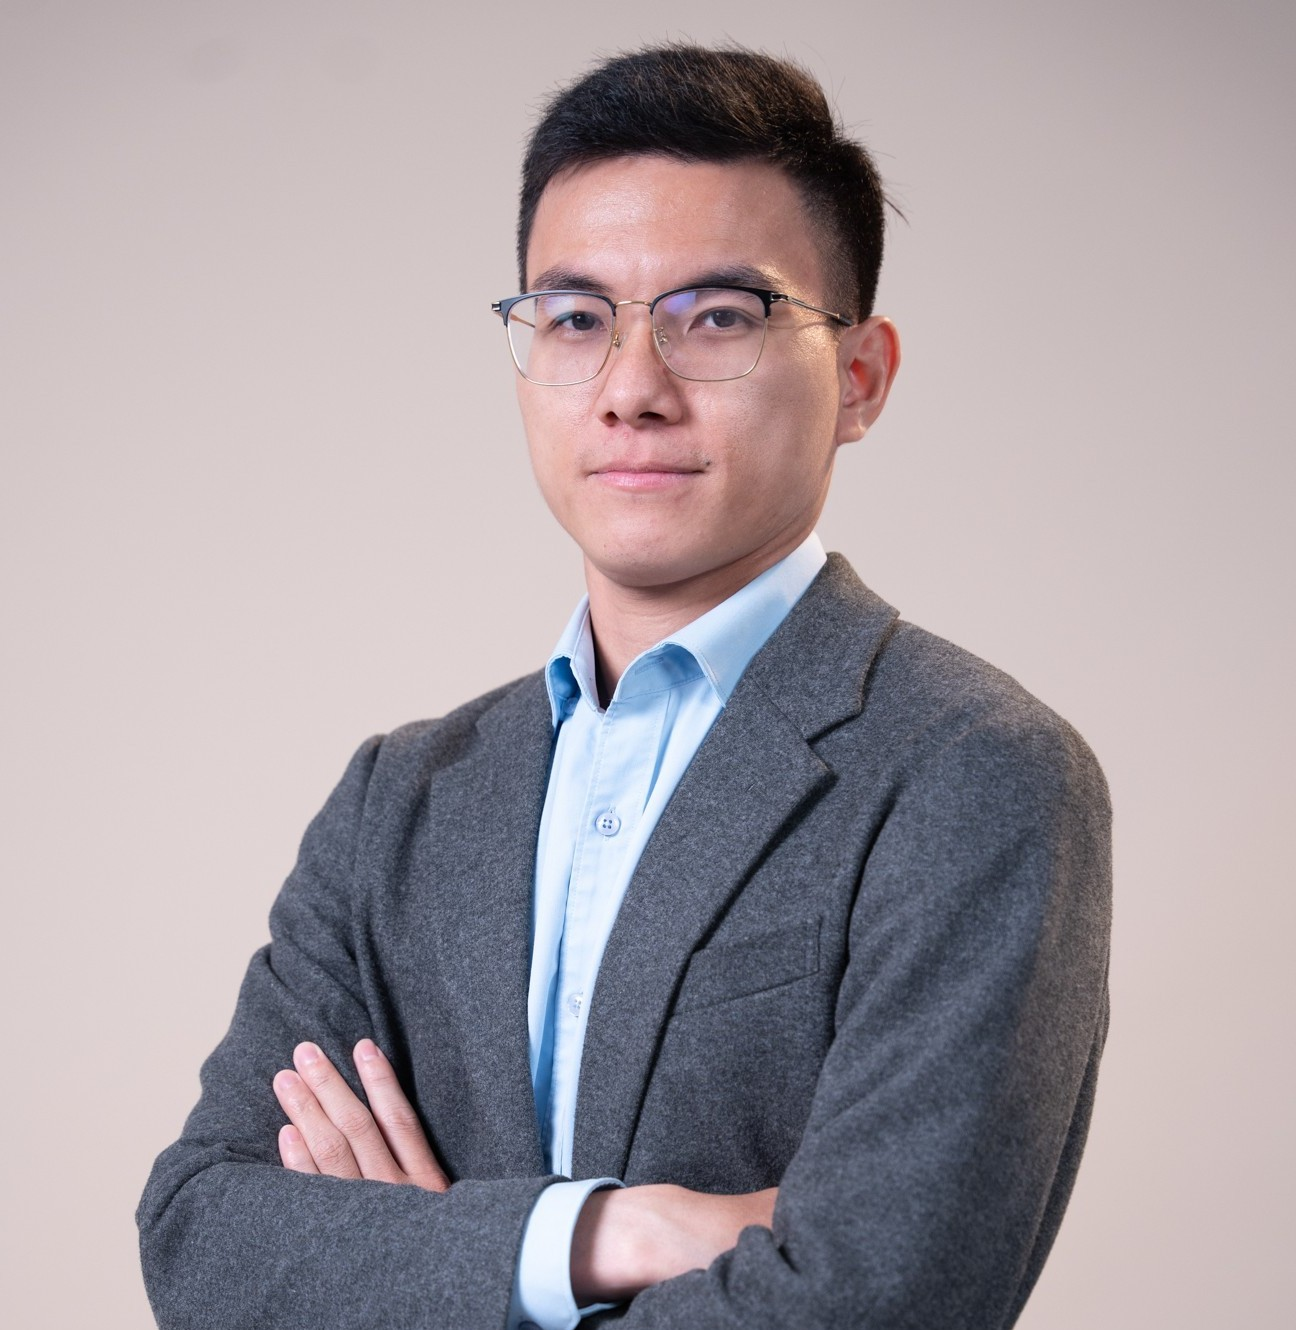
\includegraphics[width=1in,height=1.25in,clip,keepaspectratio]{authors/DinhCuong}}]{Dinh-Cuong Hoang} received his Ph.D. degree in computer science from Orebro University, Sweden (2021), and is currently a lecturer at FPT University, Greenwich Vietnam. His research interests lie at the intersection of computer vision, robotics, and machine learning. He is particularly interested in topics involving autonomy for robots, with a focus on perception algorithms.
\end{IEEEbiography}

\begin{IEEEbiography}[{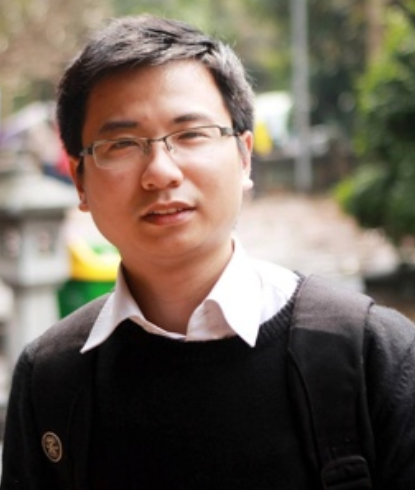
\includegraphics[width=1in,height=1.25in,clip,keepaspectratio]{authors/prof_Tan}}]{Phan Xuan Tan} (Member, IEEE) received the B.E. degree in Electrical-Electronic Engineering from Military Technical Academy, Vietnam, M.E. degree in Computer and Communication Engineering from Hanoi University of Science and Technology, Vietnam and Ph.D. degree in Functional Control Systems from Shibaura Institute of Technology, Japan. He is currently an Associate Professor at Shibaura Institute of Technology. His current research interests include computer vision, deep learning and image processing.
\end{IEEEbiography}

\begin{IEEEbiography}[{
\includegraphics[width=1in,height=1.25in,clip,keepaspectratio]{authors/NguyenAnhNhat}}]{Anh-Nhat Nguyen}  is currently a lecturer at FPT University, Vietnam. He received his B.S. and M.S. degrees in Computer Science from Duy Tan University, Da Nang, Vietnam, in 2012 and from Huazhong University of Science and Technology (HUST), China, in 2018, respectively. His research interests include image processing, information security, physical layer secrecy, radio-frequency energy harvesting, and wireless sensor networks.
\end{IEEEbiography}

\begin{IEEEbiography}[{\includegraphics[width=1in,height=1.25in,clip,keepaspectratio]{authors/TranDucThanh}}]{Duc-Thanh Tran} is pursuing a B.S. degree in Artificial Intelligence at FPT University, Hanoi, Vietnam, with a primary focus on research in the field of computer vision.
\end{IEEEbiography}

\begin{IEEEbiography}[{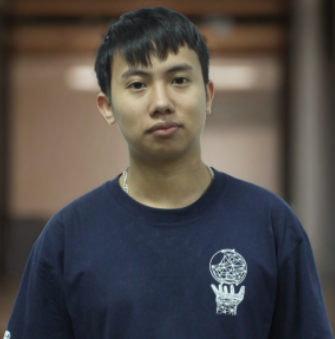
\includegraphics[width=1in,height=1.25in,clip,keepaspectratio]{authors/DuongVanHiep}}]{Van-Hiep Duong} is pursuing a B.S. degree in Artificial Intelligence at FPT University, Hanoi, Vietnam, with a primary focus on research in the field of computer vision.
\end{IEEEbiography}

\begin{IEEEbiography}[{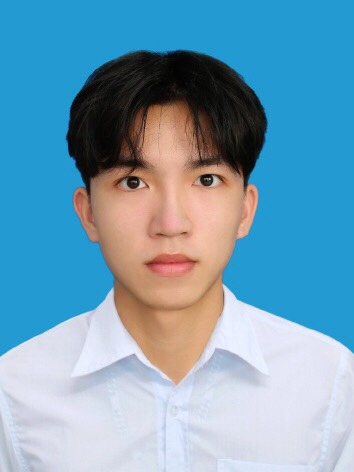
\includegraphics[width=1in,height=1.25in,clip,keepaspectratio]{authors/MaiAnhTruong}}]{Anh-Truong Mai} is pursuing a B.S. degree in Artificial Intelligence at FPT University, Hanoi, Vietnam, with a primary focus on research in the field of computer vision.
\end{IEEEbiography}

\begin{IEEEbiography}[{
\includegraphics[width=1in,height=1.25in,clip,keepaspectratio]{authors/PhamDucLong}}]{Duc-Long Pham} is pursuing a B.S. degree in Artificial Intelligence at FPT University, Hanoi, Vietnam, with a primary focus on research in the field of computer vision.
\end{IEEEbiography}

\begin{IEEEbiography}[{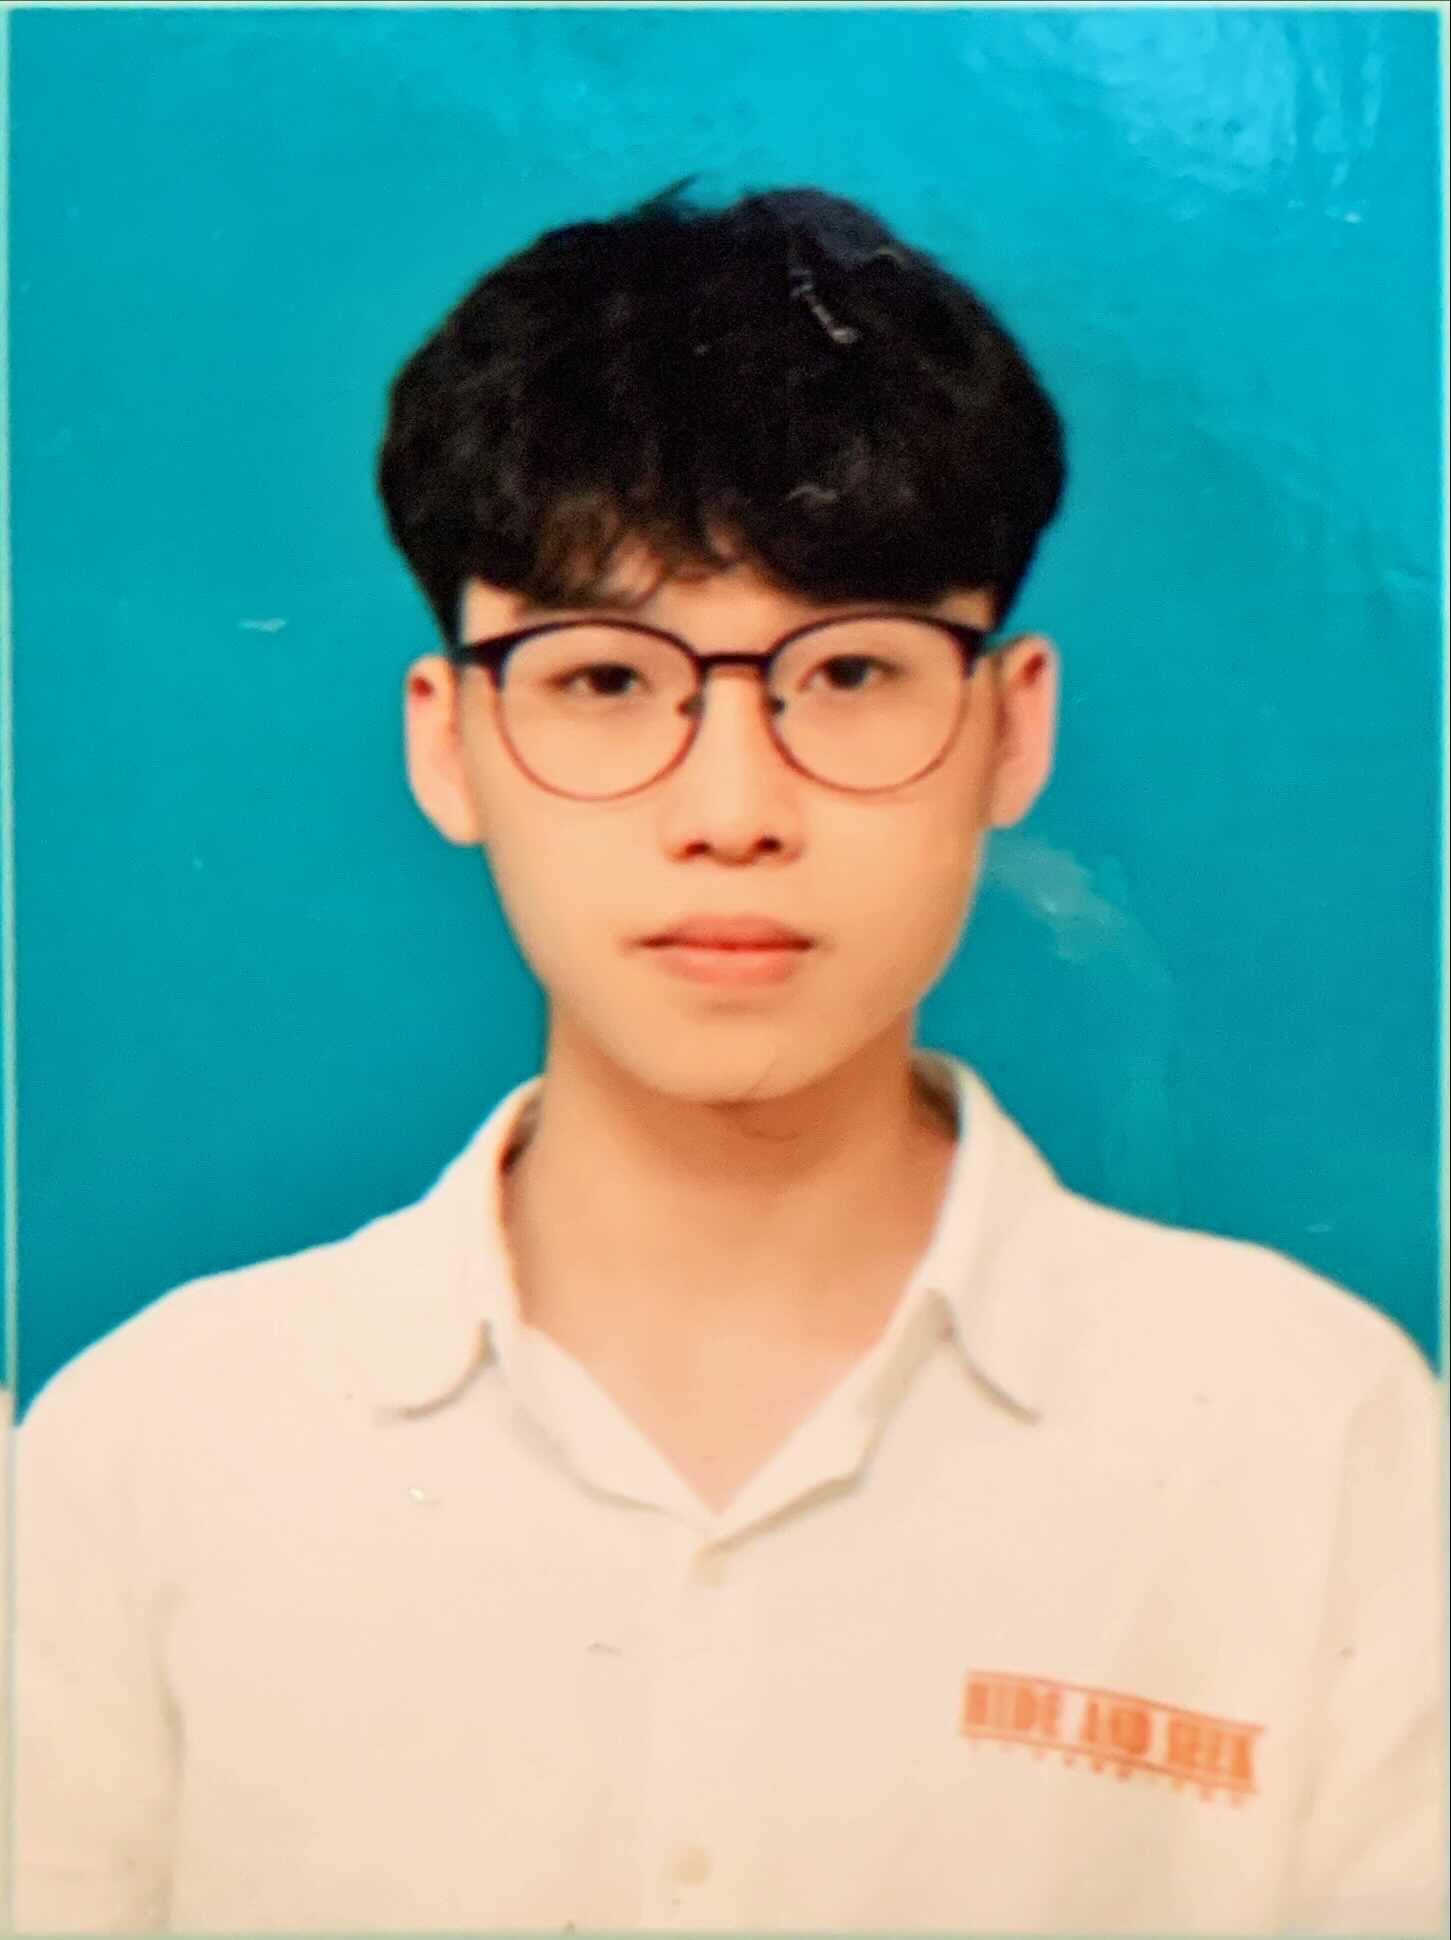
\includegraphics[width=1in,height=1.25in,clip,keepaspectratio]{authors/PhanKhanhToan}}]{Khanh-Toan Phan} is pursuing a B.S. degree in Artificial Intelligence at FPT University, Hanoi, Vietnam, with a primary focus on research in the field of computer vision.
\end{IEEEbiography}

\begin{IEEEbiography}[{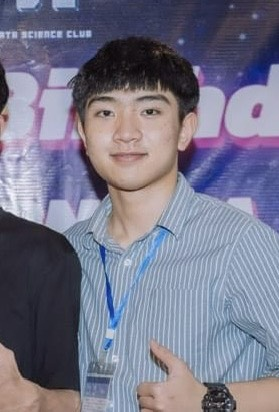
\includegraphics[width=1in,height=1.25in,clip,keepaspectratio]{authors/DoMinhQuang}}]{Minh-Quang Do} is pursuing a B.S. degree in Artificial Intelligence at FPT University, Hanoi, Vietnam, with a primary focus on research in the field of computer vision.
\end{IEEEbiography}

\begin{IEEEbiography}[{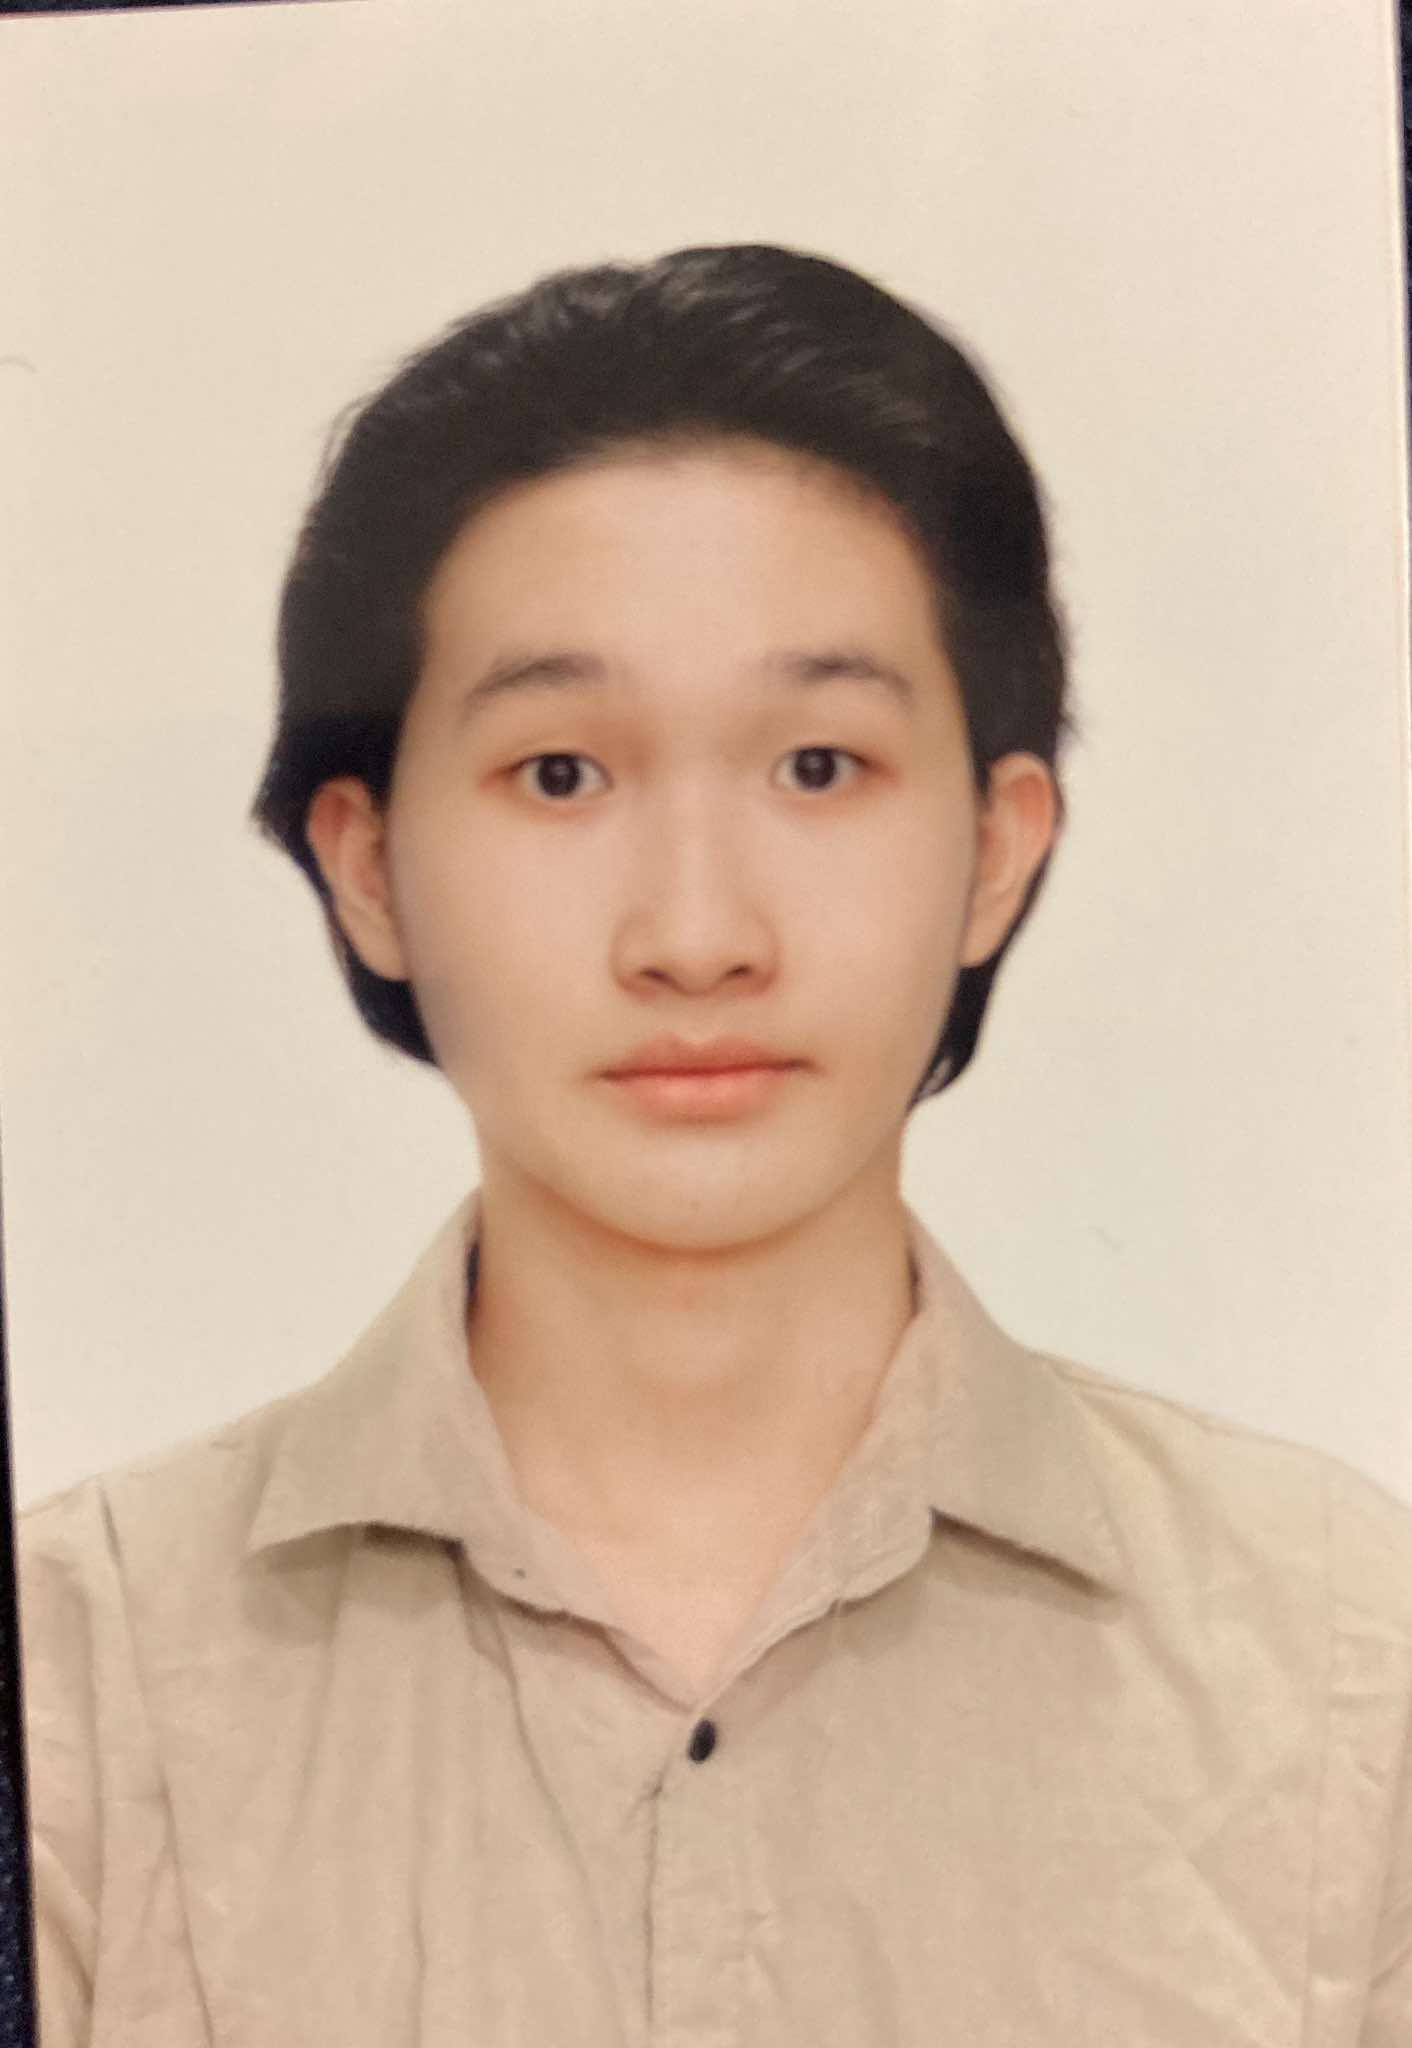
\includegraphics[width=1in,height=1.25in,clip,keepaspectratio]{authors/TaHuuAnhDuong}}]{Ta Huu Anh Duong} is pursuing a B.S. degree in Information Technology at Greenwich Vietnam, FPT University, Hanoi, Vietnam.
\end{IEEEbiography}

\begin{IEEEbiography}[{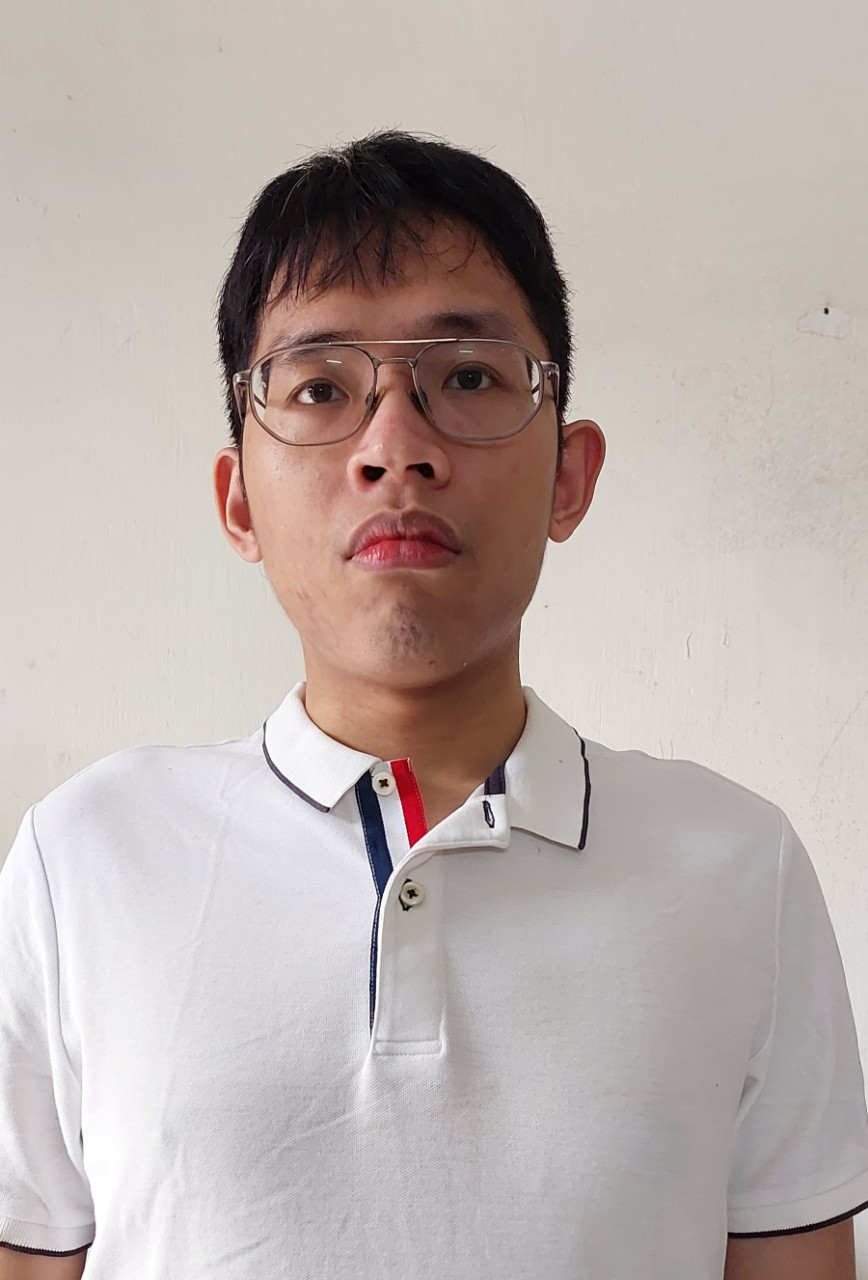
\includegraphics[width=1in,height=1.25in,clip,keepaspectratio]{authors/HuynhTuanMinh}}]{Tuan-Minh Huynh} is pursuing a B.S. degree in Information Technology at Greenwich Vietnam, FPT University, Hanoi, Vietnam.
\end{IEEEbiography}

\begin{IEEEbiography}[{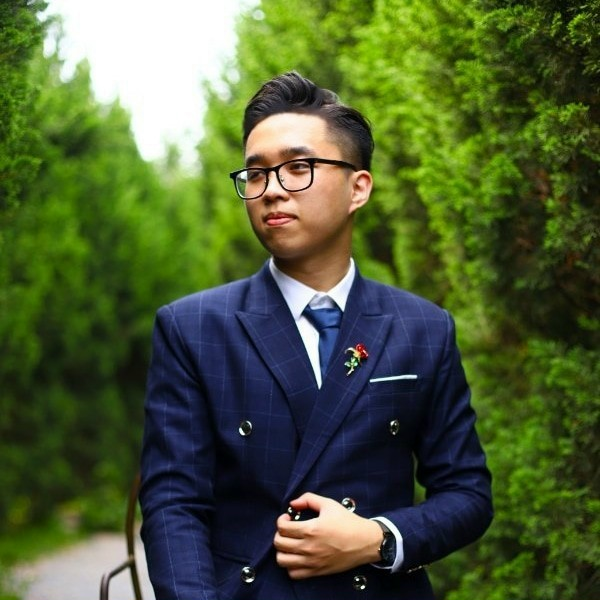
\includegraphics[width=1in,height=1.25in,clip,keepaspectratio]{authors/BuiSonAnh}}]{Son-Anh Bui} is pursuing a B.S. degree in Information Technology at Greenwich Vietnam, FPT University, Hanoi, Vietnam.
\end{IEEEbiography}

\begin{IEEEbiography}[{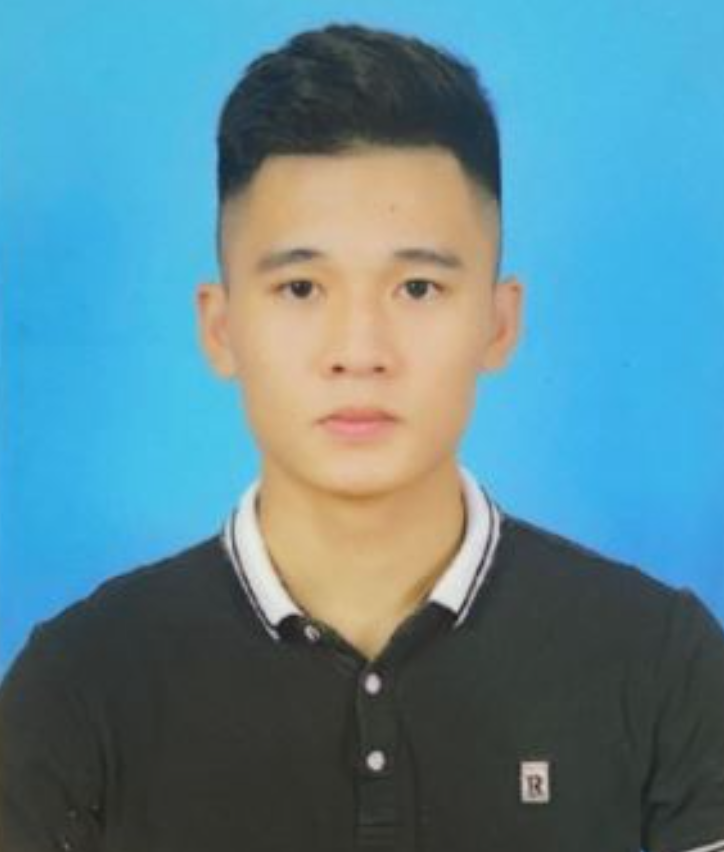
\includegraphics[width=1in,height=1.25in,clip,keepaspectratio]{authors/NguyenDucManh}}]{Duc-Manh Nguyen} is pursuing a B.S. degree in Information Technology at Greenwich Vietnam, FPT University, Hanoi, Vietnam.
\end{IEEEbiography}

\begin{IEEEbiography}[{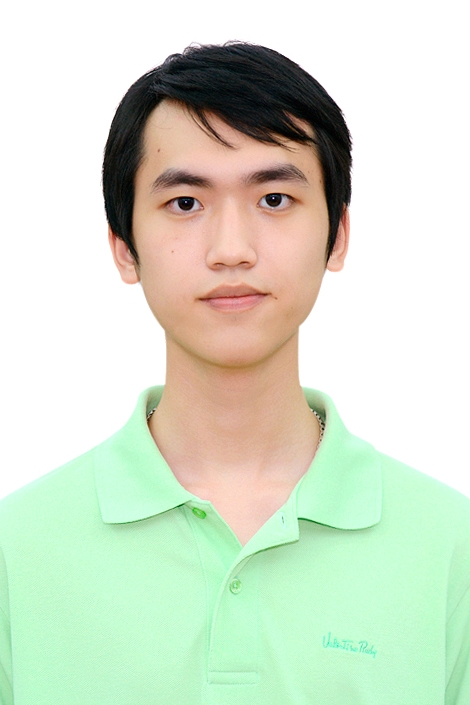
\includegraphics[width=1in,height=1.25in,clip,keepaspectratio]{authors/TrinhVietAnh}}]{Viet-Anh Trinh} is pursuing a B.S. degree in Information Technology at Greenwich Vietnam, FPT University, Hanoi, Vietnam.
\end{IEEEbiography}

\begin{IEEEbiography}[{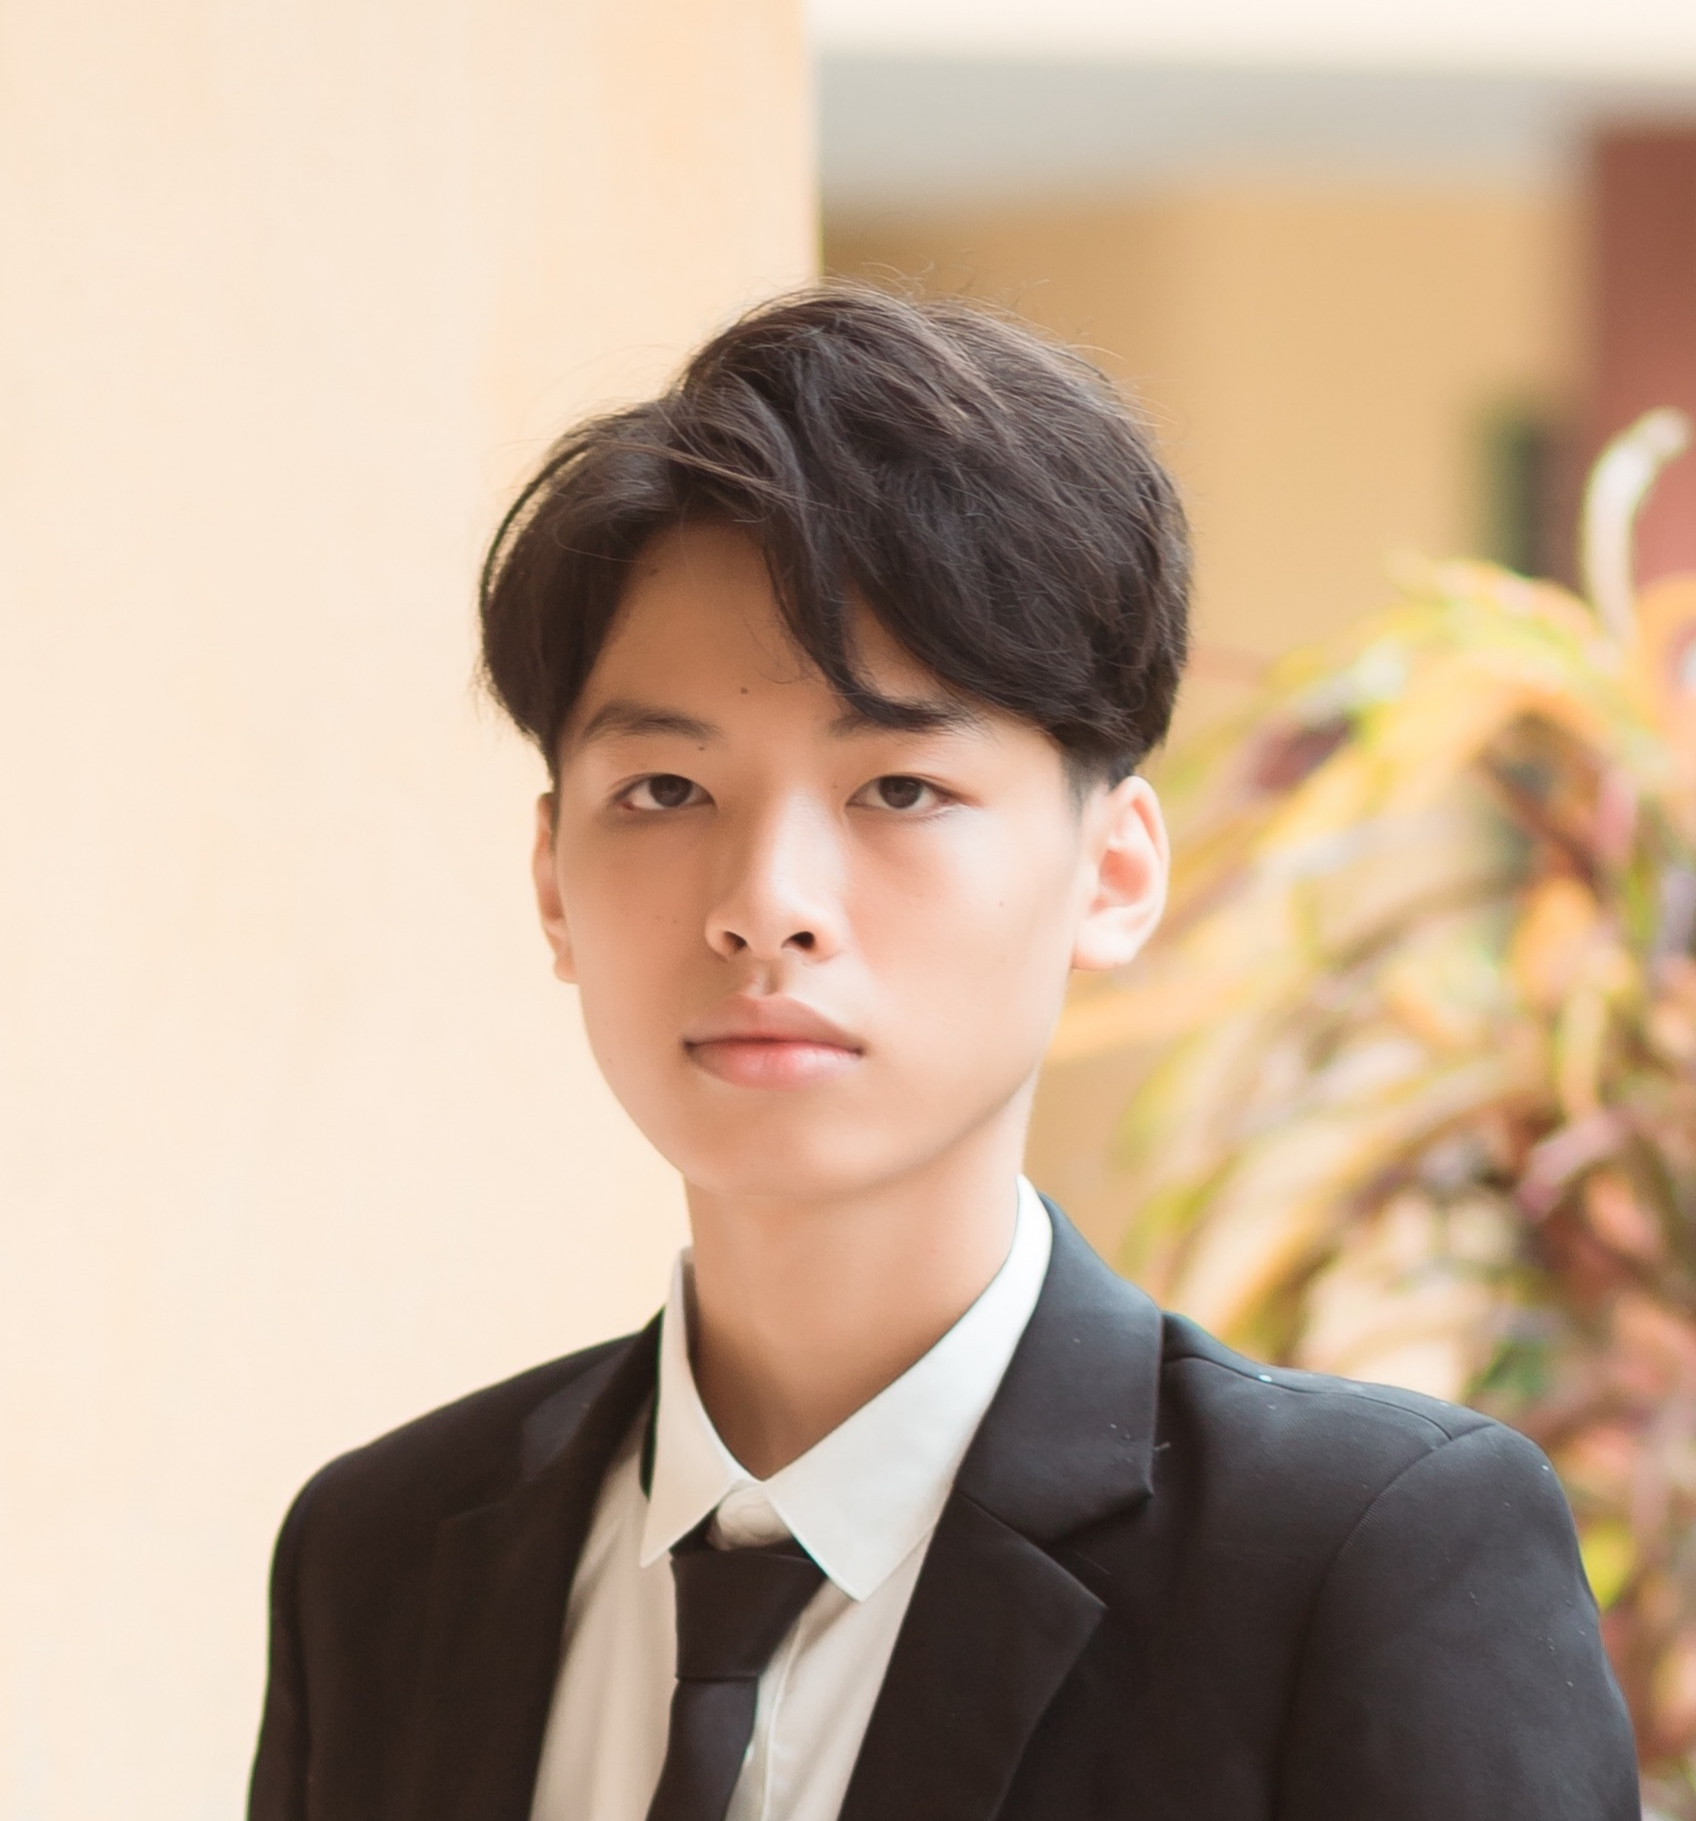
\includegraphics[width=1in,height=1.25in,clip,keepaspectratio]{authors/TranKhanhDuong}}]{Khanh-Duong Tran} is pursuing a B.S. degree in Information Technology at Greenwich Vietnam, FPT University, Hanoi, Vietnam.
\end{IEEEbiography}

\EOD

\end{document}
